% Options for packages loaded elsewhere
% Options for packages loaded elsewhere
\PassOptionsToPackage{unicode}{hyperref}
\PassOptionsToPackage{hyphens}{url}
\PassOptionsToPackage{dvipsnames,svgnames,x11names}{xcolor}
%
\documentclass[
  letterpaper,
  DIV=11,
  numbers=noendperiod]{scrartcl}
\usepackage{xcolor}
\usepackage[top=30mm,left=30mm]{geometry}
\usepackage{amsmath,amssymb}
\setcounter{secnumdepth}{-\maxdimen} % remove section numbering
\usepackage{iftex}
\ifPDFTeX
  \usepackage[T1]{fontenc}
  \usepackage[utf8]{inputenc}
  \usepackage{textcomp} % provide euro and other symbols
\else % if luatex or xetex
  \usepackage{unicode-math} % this also loads fontspec
  \defaultfontfeatures{Scale=MatchLowercase}
  \defaultfontfeatures[\rmfamily]{Ligatures=TeX,Scale=1}
\fi
\usepackage{lmodern}
\ifPDFTeX\else
  % xetex/luatex font selection
\fi
% Use upquote if available, for straight quotes in verbatim environments
\IfFileExists{upquote.sty}{\usepackage{upquote}}{}
\IfFileExists{microtype.sty}{% use microtype if available
  \usepackage[]{microtype}
  \UseMicrotypeSet[protrusion]{basicmath} % disable protrusion for tt fonts
}{}
\makeatletter
\@ifundefined{KOMAClassName}{% if non-KOMA class
  \IfFileExists{parskip.sty}{%
    \usepackage{parskip}
  }{% else
    \setlength{\parindent}{0pt}
    \setlength{\parskip}{6pt plus 2pt minus 1pt}}
}{% if KOMA class
  \KOMAoptions{parskip=half}}
\makeatother
% Make \paragraph and \subparagraph free-standing
\makeatletter
\ifx\paragraph\undefined\else
  \let\oldparagraph\paragraph
  \renewcommand{\paragraph}{
    \@ifstar
      \xxxParagraphStar
      \xxxParagraphNoStar
  }
  \newcommand{\xxxParagraphStar}[1]{\oldparagraph*{#1}\mbox{}}
  \newcommand{\xxxParagraphNoStar}[1]{\oldparagraph{#1}\mbox{}}
\fi
\ifx\subparagraph\undefined\else
  \let\oldsubparagraph\subparagraph
  \renewcommand{\subparagraph}{
    \@ifstar
      \xxxSubParagraphStar
      \xxxSubParagraphNoStar
  }
  \newcommand{\xxxSubParagraphStar}[1]{\oldsubparagraph*{#1}\mbox{}}
  \newcommand{\xxxSubParagraphNoStar}[1]{\oldsubparagraph{#1}\mbox{}}
\fi
\makeatother


\usepackage{longtable,booktabs,array}
\newcounter{none} % for unnumbered tables
\usepackage{calc} % for calculating minipage widths
% Correct order of tables after \paragraph or \subparagraph
\usepackage{etoolbox}
\makeatletter
\patchcmd\longtable{\par}{\if@noskipsec\mbox{}\fi\par}{}{}
\makeatother
% Allow footnotes in longtable head/foot
\IfFileExists{footnotehyper.sty}{\usepackage{footnotehyper}}{\usepackage{footnote}}
\makesavenoteenv{longtable}
\usepackage{graphicx}
\makeatletter
\newsavebox\pandoc@box
\newcommand*\pandocbounded[1]{% scales image to fit in text height/width
  \sbox\pandoc@box{#1}%
  \Gscale@div\@tempa{\textheight}{\dimexpr\ht\pandoc@box+\dp\pandoc@box\relax}%
  \Gscale@div\@tempb{\linewidth}{\wd\pandoc@box}%
  \ifdim\@tempb\p@<\@tempa\p@\let\@tempa\@tempb\fi% select the smaller of both
  \ifdim\@tempa\p@<\p@\scalebox{\@tempa}{\usebox\pandoc@box}%
  \else\usebox{\pandoc@box}%
  \fi%
}
% Set default figure placement to htbp
\def\fps@figure{htbp}
\makeatother


% definitions for citeproc citations
\NewDocumentCommand\citeproctext{}{}
\NewDocumentCommand\citeproc{mm}{%
  \begingroup\def\citeproctext{#2}\cite{#1}\endgroup}
\makeatletter
 % allow citations to break across lines
 \let\@cite@ofmt\@firstofone
 % avoid brackets around text for \cite:
 \def\@biblabel#1{}
 \def\@cite#1#2{{#1\if@tempswa , #2\fi}}
\makeatother
\newlength{\cslhangindent}
\setlength{\cslhangindent}{1.5em}
\newlength{\csllabelwidth}
\setlength{\csllabelwidth}{3em}
\newenvironment{CSLReferences}[2] % #1 hanging-indent, #2 entry-spacing
 {\begin{list}{}{%
  \setlength{\itemindent}{0pt}
  \setlength{\leftmargin}{0pt}
  \setlength{\parsep}{0pt}
  % turn on hanging indent if param 1 is 1
  \ifodd #1
   \setlength{\leftmargin}{\cslhangindent}
   \setlength{\itemindent}{-1\cslhangindent}
  \fi
  % set entry spacing
  \setlength{\itemsep}{#2\baselineskip}}}
 {\end{list}}
\usepackage{calc}
\newcommand{\CSLBlock}[1]{\hfill\break\parbox[t]{\linewidth}{\strut\ignorespaces#1\strut}}
\newcommand{\CSLLeftMargin}[1]{\parbox[t]{\csllabelwidth}{\strut#1\strut}}
\newcommand{\CSLRightInline}[1]{\parbox[t]{\linewidth - \csllabelwidth}{\strut#1\strut}}
\newcommand{\CSLIndent}[1]{\hspace{\cslhangindent}#1}



\setlength{\emergencystretch}{3em} % prevent overfull lines

\providecommand{\tightlist}{%
  \setlength{\itemsep}{0pt}\setlength{\parskip}{0pt}}



 


\KOMAoption{captions}{tableheading}
\makeatletter
\@ifpackageloaded{tcolorbox}{}{\usepackage[skins,breakable]{tcolorbox}}
\@ifpackageloaded{fontawesome5}{}{\usepackage{fontawesome5}}
\definecolor{quarto-callout-color}{HTML}{909090}
\definecolor{quarto-callout-note-color}{HTML}{0758E5}
\definecolor{quarto-callout-important-color}{HTML}{CC1914}
\definecolor{quarto-callout-warning-color}{HTML}{EB9113}
\definecolor{quarto-callout-tip-color}{HTML}{00A047}
\definecolor{quarto-callout-caution-color}{HTML}{FC5300}
\definecolor{quarto-callout-color-frame}{HTML}{acacac}
\definecolor{quarto-callout-note-color-frame}{HTML}{4582ec}
\definecolor{quarto-callout-important-color-frame}{HTML}{d9534f}
\definecolor{quarto-callout-warning-color-frame}{HTML}{f0ad4e}
\definecolor{quarto-callout-tip-color-frame}{HTML}{02b875}
\definecolor{quarto-callout-caution-color-frame}{HTML}{fd7e14}
\makeatother
\makeatletter
\@ifpackageloaded{caption}{}{\usepackage{caption}}
\AtBeginDocument{%
\ifdefined\contentsname
  \renewcommand*\contentsname{Table of contents}
\else
  \newcommand\contentsname{Table of contents}
\fi
\ifdefined\listfigurename
  \renewcommand*\listfigurename{List of Figures}
\else
  \newcommand\listfigurename{List of Figures}
\fi
\ifdefined\listtablename
  \renewcommand*\listtablename{List of Tables}
\else
  \newcommand\listtablename{List of Tables}
\fi
\ifdefined\figurename
  \renewcommand*\figurename{Figure}
\else
  \newcommand\figurename{Figure}
\fi
\ifdefined\tablename
  \renewcommand*\tablename{Table}
\else
  \newcommand\tablename{Table}
\fi
}
\@ifpackageloaded{float}{}{\usepackage{float}}
\floatstyle{ruled}
\@ifundefined{c@chapter}{\newfloat{codelisting}{h}{lop}}{\newfloat{codelisting}{h}{lop}[chapter]}
\floatname{codelisting}{Listing}
\newcommand*\listoflistings{\listof{codelisting}{List of Listings}}
\makeatother
\makeatletter
\makeatother
\makeatletter
\@ifpackageloaded{caption}{}{\usepackage{caption}}
\@ifpackageloaded{subcaption}{}{\usepackage{subcaption}}
\makeatother
\makeatletter
\@ifpackageloaded{fontawesome6}{}{\usepackage{fontawesome6}}
\makeatother
\usepackage{bookmark}
\IfFileExists{xurl.sty}{\usepackage{xurl}}{} % add URL line breaks if available
\urlstyle{same}
\hypersetup{
  pdftitle={Threats to credible research: Where are we at?},
  pdfauthor={Sarah von Grebmer zu Wolfsthurn},
  colorlinks=true,
  linkcolor={blue},
  filecolor={Maroon},
  citecolor={Blue},
  urlcolor={Blue},
  pdfcreator={LaTeX via pandoc}}


\title{Threats to credible research: Where are we at?}
\author{Sarah von Grebmer zu Wolfsthurn}
\date{17/04/2026}
\begin{document}
\maketitle


\subsection{Licence}\label{licence}

This work was originally created by
\href{https://www.nicebread.de/}{Felix Schönbrodt} under a CC-BY 4.0
\href{https://creativecommons.org/licenses/by/4.0/deed.en}{Creative
Commons Attribution 4.0 International License}. This current work by
Sarah von Grebmer zu Wolfsthurn, Malika Ihle and Felix Schönbrodt is
licensed under a CC-BY-SA 4.0
\href{https://creativecommons.org/licenses/by-sa/4.0/deed.en}{Creative
Commons Attribution 4.0 International SA License}. It permits
unrestricted re-use, distribution, and reproduction in any medium,
provided the original work is properly cited. If you remix, transform,
or build upon the material, you must distribute your contributions under
the same license as the original.

\textbf{Presenter Notes}: The Creative Commons Attribution--ShareAlike
4.0 license, or CC BY-SA 4.0, allows others to copy, share, and adapt a
work in any medium, including for commercial purposes. These permissions
are broad and cannot be withdrawn as long as the license terms are
followed. The main requirement is attribution: users must give
appropriate credit to the original creator, provide a link to the
license, and clearly indicate whether any changes were made, without
implying endorsement by the original author. In addition, the ShareAlike
condition means that if someone modifies or builds upon the work, the
resulting material must be distributed under the same CC BY-SA 4.0
license, or a compatible one. Finally, users are not allowed to apply
legal or technical restrictions, such as DRM, that would prevent others
from exercising these same rights.

\subsection{Contribution statement}\label{contribution-statement}

\textbf{Creator}: Von Grebmer zu Wolfsthurn, Sarah
(\pandocbounded{
\includegraphics[keepaspectratio]{images/ORCID-iD_icon_16x16.png}}
\href{https://orcid.org/0000-0002-6413-3895}{0000-0002-6413-3895})

\textbf{Reviewer}: Schönbrodt, Felix
(\pandocbounded{
\includegraphics[keepaspectratio]{images/ORCID-iD_icon_16x16.png}}\href{https://orcid.org/0000-0002-8282-3910}{0000-0002-8282-3910})

\textbf{Consultant}: Ihle, Malika
(\pandocbounded{
\includegraphics[keepaspectratio]{images/ORCID-iD_icon_16x16.png}}
\href{https://orcid.org/0000-0002-3242-5981}{0000-0002-3242-5981})

\textbf{Presenter Notes}: These are the \textbf{presenter notes}. You
will a script for the presenter for every slide. In presentation mode,
your audience will not be able to see these presenter notes, they are
only visible to the presenter.

\textbf{Instructor Notes}: There are also \textbf{instructor notes}. For
some slides, there will be pedagogical tips, suggestions for activities
and troubleshooting tips for issues your audience might run into. You
can find these notes underneath the presenter notes.

\textbf{Acessibility Tips}: Where applicable, this is a space to add any
tips you may have to facilitate the accessibility of your slides and
activities.

\subsection{Prerequisites}\label{prerequisites}

\begin{tcolorbox}[enhanced jigsaw, arc=.35mm, bottomrule=.15mm, bottomtitle=1mm, breakable, colback=white, colbacktitle=quarto-callout-important-color!10!white, colframe=quarto-callout-important-color-frame, coltitle=black, left=2mm, leftrule=.75mm, opacityback=0, opacitybacktitle=0.6, rightrule=.15mm, title=\textcolor{quarto-callout-important-color}{\faExclamation}\hspace{0.5em}{Important}, titlerule=0mm, toprule=.15mm, toptitle=1mm]

Before completing this submodule, please carefully read about the
prerequisites.

\end{tcolorbox}

{\def\LTcaptype{none} % do not increment counter
\begin{longtable}[]{@{}
  >{\raggedright\arraybackslash}p{(\linewidth - 4\tabcolsep) * \real{0.3333}}
  >{\raggedright\arraybackslash}p{(\linewidth - 4\tabcolsep) * \real{0.3333}}
  >{\raggedright\arraybackslash}p{(\linewidth - 4\tabcolsep) * \real{0.3333}}@{}}
\toprule\noalign{}
\begin{minipage}[b]{\linewidth}\raggedright
Prerequisite
\end{minipage} & \begin{minipage}[b]{\linewidth}\raggedright
Description
\end{minipage} & \begin{minipage}[b]{\linewidth}\raggedright
Link/Where to find it
\end{minipage} \\
\midrule\noalign{}
\endhead
\bottomrule\noalign{}
\endlastfoot
UNESCO Recommendations on Open Science & Recommended reading: pp 6-19 &
\href{https://unesdoc.unesco.org/ark:/48223/pf0000379949}{Download
Link} \\
\end{longtable}
}

\textbf{Presenter Notes}: Since this is the introductory submodule of
this module, there are no formal prerequisites for this session. If you
will, today we are all starting on a blank page. The UNESCO
Recommendation on Open Science is an optional prerequisite which sets
the scene for what this course will be all about. The UNESCO
Recommendation on Open Science is a landmark international framework
adopted by UNESCO Member States in November 2021. It represents the
first global standard-setting instrument for open research. The
recommendation provides a shared definition, core values, guiding
principles, and a set of action areas designed to help shape policies
and practices that make science more accessible, transparent, inclusive,
and equitable. Reading at least part of the recommendations before
starting this course can provide a global context and shared language
for understanding the concepts and goals that underlie open science
practices. This helps ensure discussions are grounded in internationally
recognized standards. It also clarifies the broad scope of open science,
which goes beyond open access to publications and data to include
cultural change, policy, education, societal engagement, and ethical
considerations. The recommendations highlight the rationale and
potential impact of open science, particularly in terms of equity,
inclusiveness, and the capacity to address complex global challenges
through enhanced collaboration and information sharing.

\textbf{Instructor Notes}: Since this is the introductory submodule of
this module, there are no formal prerequisites. However, to get a small
kick-start into the topic, learners are advised to have skimmed the
UNESCO Recommendations on Open Science, particularly pages 6-19.

\subsection{Threats to credible research - Intro
Survey}\label{threats-to-credible-research---intro-survey}

\textbf{Presenter Notes}: Before we get started, I would like to explore
your previous knowledge around Open Research. Perhaps some of you have
read the recommedations by UNESCO, perhaps some have never heard of the
term Open Research before. On the following slides you will find some
questions which aim to capture how much you know already. You can scan
the QR code, which will take you to a survey tool where you can click
your way through the questions. We will then briefly discuss the
questions in the plenum. Some of these questions I will ask again
towards the end of this session, to get an understanding of whether
anything has changed in terms of your knowledge or understanding during
this session.

\textbf{Instructor Notes}:

\begin{itemize}
\item
  \textbf{Aim}: The pre-submodule survey serves to examine students'
  prior knowledge about the submodule's topic.
\item
  Use free survey software such as Particify to establish the following
  questions (shown on separate slides).
\item
  \emph{Note}: This survey component does not work in an asynchronous
  setting.
\end{itemize}

\subsection{Survey}\label{survey}

\textbf{Based on your experience so far, how would you currently rate
your trust in published scientific findings on a scale from 1 - 5?}

\begin{itemize}
\tightlist
\item
  1 = trusting virtually \textbf{none} of the findings
\item
  2 = trusting only \textbf{some} findings
\item
  3 = trusting about \textbf{half} of the findings
\item
  4 = trusting the \textbf{majority} of the findings
\item
  5 = trusting virtually \textbf{all} findings
\end{itemize}

\subsection{Survey}\label{survey-1}

\textbf{Based on your experience so far, which challenges to research
trustworthiness do you see? Name a few keywords.}

Display Wordcloud answer.

\subsection{Survey}\label{survey-2}

\textbf{Based on your experience so far, which concepts do you connect
to research more broadly?}

Display Wordcloud answer.

\subsection{Survey}\label{survey-3}

\textbf{What is your level of familiarity with Open Research practices
in general (e.g., basic concepts, terminology, or tools)?}

\begin{enumerate}
\def\labelenumi{\alph{enumi}.}
\item
  I am unfamiliar with the concept of Open Research practices.
\item
  I have heard of them but I would not know how they apply to my work.
\item
  I have basic understanding and experience with Open Research practices
  in my own work/research/studies.
\item
  I am very familiar with Open Research practices and routinely apply
  them in my daily work/research/study routines.
\end{enumerate}

\subsection{Discussion of survey
results}\label{discussion-of-survey-results}

What do we see in the results?

\textbf{Presenter Notes}: Script for the slide here.

\textbf{Instructor Notes}:

\begin{itemize}
\item
  \textbf{Aim''}: Briefly examine the answers given to each question
  interactively with the group.
\item
  Use visuals from the survey to highlight specific answers.
\end{itemize}

\subsection{\texorpdfstring{\faIcon{people-group} Your current
understanding of key terms (6
min)}{ Your current understanding of key terms (6 min)}}\label{b58fc729-690b-4000-b19f-365a4093b2ff7b7b3c2066612070656f706c652d67726f75702073697a653d3178203e7d7d-your-current-understanding-of-key-terms-6-min}

\subsubsection{Think - Pair - Share}\label{think---pair---share}

\begin{itemize}
\tightlist
\item
  \textbf{Think} (2 min): For yourself: Write down a definition for the
  key terms listed below {(without internet search - your current
  understanding)}
\item
  \textbf{Pair} (2 min): Discuss your definitions with your neighbour
\item
  \textbf{Share} (2 min): Share your definitions with the larger group
\end{itemize}

\subsection{Covered in this session}\label{covered-in-this-session}

\begin{itemize}
\tightlist
\item
  \textbf{Do} people \textbf{trust} in science?
\item
  \textbf{Should} people \textbf{trust} in science? Replicability and
  reproducibilty
\item
  Threats to replicability: \textbf{p-hacking, errors, and biases} in
  research
\end{itemize}

\textbf{Presenter Notes}: This slide provides an overview of the main
topics we will cover in this session. Do not worry if some of these
concepts make no sense to you at this point, we will get to all of them
by the end of this session. We will begin by looking at research and the
research cycle. We will look at how knowledge is produced, from forming
a research question, through data collection and analysis, to
publication and dissemination. Next, we will discuss trust in research
and what it means. Trust is fundamental to science and research because
it shapes how researchers trust each other's work, how institutions make
decisions based on evidence, and how society at large engages with
scientific findings. We will then move on to replicability and
reproducibility, two key concepts for assessing the robustness of
research. We will clarify the difference between them and examine why
the inability to replicate or reproduce results has become a major
concern across many disciplines. Following that, we will learn about
biases, inconsistencies, and mistakes in research. These issues are
often unintentional but can arise from methodological choices, data
handling, publication pressures, or systemic incentives. Recognizing
these challenges helps us better understand where and why research can
go wrong.

\textbf{Instructor Notes}: Add.

\subsection{Learning goals}\label{learning-goals}

By the end of this session, learners will be able to:

\begin{itemize}
\tightlist
\item
  \textbf{Define} and \textbf{distinguish} key terms related to
  research, including research cycle, trust in research, replicability,
  reproducibility, and open research
\item
  \textbf{Recognize} different types of challenges in research: research
  biases, statistical insecurities, errors and where they can arise from
\item
  \textbf{Analyze} research scenarios to identify potential research
  biases and questionable research practices
\item
  \textbf{Reflect} on the current threats for research and on the need
  for alternative approaches to conducting research
\end{itemize}

\textbf{Presenter Notes}: Script for the slide here.

\textbf{Instructor Notes}:

\begin{itemize}
\item
  \textbf{Aim}: Formulate specific, action-oriented goals learning goals
  which are measurable and observable in line with Bloom's taxonomy
  (Anderson \& Krathwohl, 2001; Bloom, 1956)
\item
  Place an emphasis on the \textbf{verbs} of the learning goals and
  choose verbs that align with the skills you want to develop or assess.
\item
  Examples:

  \begin{itemize}
  \tightlist
  \item
    Students will \textbf{describe} the process of photosynthesis or
  \item
    Students will \textbf{construct} a diagram illustrating the process
    of photosynthesis
  \end{itemize}
\end{itemize}

\section{Do people trust in
research?}\label{do-people-trust-in-research}

\subsection{What is public ``trust'' in
research?}\label{what-is-public-trust-in-research}

\begin{itemize}
\item
  ``\emph{Society trusts that scientific research results are an honest
  and accurate reflection of a researcher's work.}'' {(Committee on
  Science, Engineering and Public Policy 2009: ix)}
\item
  ``\emph{The public must be able to trust the science and scientific
  process informing public policy decisions.}'' {(Obama 2009)}
\end{itemize}

Resnik, D. B. (2011). Scientific research and the public trust.
\emph{Science and engineering ethics, 17}(3), 399-409.

\textbf{Presenter Notes}: What do we mean by trust in research? In their
paper, Resnik argues that maintaining public trust is essential for the
scientific enterprise, and he highlights how U.S. policy leaders have
emphasized this responsibility. For example, he references the 2009
Committee on Science and Technology report, which highlights that the
public expects science to be conducted responsibly and that preserving
trust requires strong ethical norms, oversight, and systems that prevent
misconduct. The part on ``honest reflection of a researcher's work is
particularly central here: society should be able to get a reliable and
truthful insight into the methods and outcomes of the research process.
They also cite President Obama's 2009 statement on scientific integrity,
which stresses that government science must be guided by facts,
transparency, and freedom from political manipulation. Resnik uses this
to illustrate that public trust in science and research is not
automatic. Going even further, they argue that trust needs to be earned
and protected, given that science and research play a critical role in
informing policies relevant to the public.

\textbf{Instructor Notes}: Beware that depending on the background of
your learners, trust can have many facets. At its core, trust refers to
the confidence that research processes, findings, and actors are
reliable, ethical, and credible. However, how this trust is understood
and emphasized can vary by discipline and fields. One important
dimension of trust relates to research methods. Across scientific
disciplines, trust is built when appropriate methods are chosen, data
are collected and analyzed rigorously, and decisions are clearly
justified. In \textbf{experimental and quantitative fields}, this often
involves standardized procedures, controls, and statistical robustness.
In qualitative and interpretive disciplines, trust may instead be
grounded in transparency, reflexivity, and the coherence of the research
design. Another dimension is trust in researchers and research
communities. This includes expectations of integrity, honesty, and
adherence to ethical standards, as well as openness about limitations
and potential conflicts of interest. In \textbf{research involving human
participants or sensitive topics}, trust is closely linked to ethical
responsibility and respect for participants. Trust also concerns
research results and findings. This involves confidence that conclusions
are supported by evidence and have not been distorted through selective
reporting or questionable practices. Concepts such as replicability and
reproducibility play a key role here, particularly in fields where
results are expected to be independently verified. In \textbf{applied
research areas such as medicine, engineering, or economics}, trust in
findings is especially critical because research outcomes directly
influence decisions, policies, and interventions. These dimensions are
good to keep in mind when interacting with your learners.

\subsection{Measuring trust in
research}\label{measuring-trust-in-research}

\faIcon{chart-bar} Probe your prejudices: In which profession do you
have the highest trust to tell the truth? And the lowest?

. . .

{Data from 1,015 UK adults, 2024}

Sources: Veracity Index 2024,
\href{https://www.ipsos.com/en\%2Duk/ipsos\%2Dveracity\%2Dindex\%2D2024}{Ipsos};
Seyd, B. (2025). What is trust (in science and scientists) and is it in
crisis?. \emph{Current Opinion in Psychology, 67}.
\url{https://doi.org/10.1016/j.copsyc.2025.102201}

\textbf{Presenter Notes}: This chart shows results from the Ipsos
Veracity Index 2024, which measures how much the UK public trusts
different professions to tell the truth. The findings are based on a
nationally representative sample of around 1,000 UK adults. Respondents
were asked how much they trust people in each profession to tell the
truth, and the chart reports the percentage who say they trust them
(either ``a great deal'' or ``a fair amount'').

Starting at the top, nurses are the most trusted profession, with very
high trust levels. They are followed closely by engineers and doctors,
and then teachers and professors. Scientists also score relatively high,
just behind judges and museum curators. These top professions share a
common theme: they are generally seen as skilled, evidence-based, and
working in the public interest, which likely contributes to their high
trust. Moving to the middle of the chart, we see professions like
police, judges, and business leaders, where trust is more moderate and
mixed. At the lower end, journalists and advertising executives have
relatively low trust levels. Finally, politicians and government
ministers are the least trusted, with a significant gap between them and
the top-ranked professions.

\subsection{Public trust in research}\label{public-trust-in-research}

\subsubsection{German survey
``Wissenschaftsbarometer''}\label{german-survey-wissenschaftsbarometer}

\pandocbounded{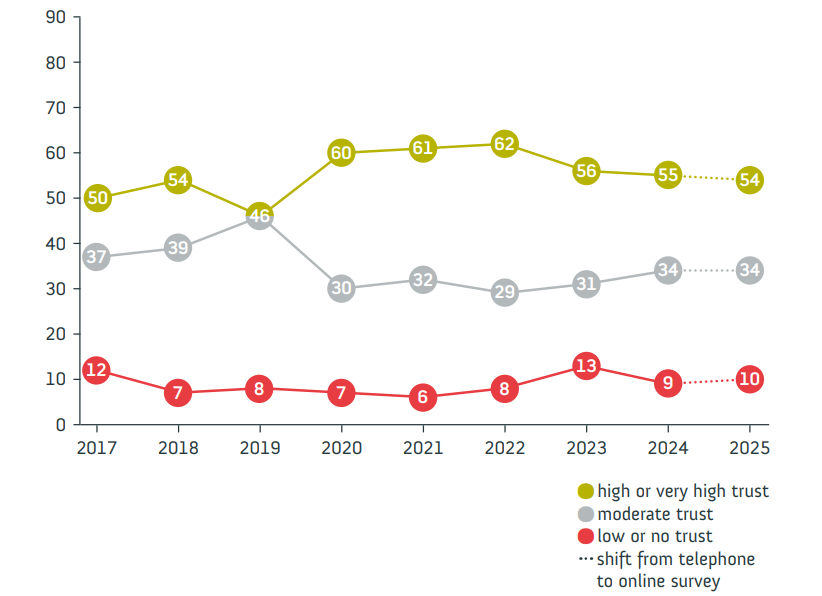
\includegraphics[keepaspectratio]{images/public_trust_in_science.png}}

Source: \emph{Wissenschaft im Dialog/Verian}:
\url{www.sciencebarometer.com}.

\textbf{Presenter Notes}: Let us have a look at trust in research from
the perspective of the general public. The Science Barometer is an
annual survey of the German general public's attitudes toward science
and research. It has been conducted every year since 2014 by
Wissenschaft im Dialog (WiD). It focuses on a number of different
elements, such as the expectations towards science, the relevance of
science but also the trustworthiness of research and science. It is
conducted annually and targets the German-speaking population aged 14
and over living in private households in Germany. The survey was
traditionally conducted over the phone, but in 2025 shifted to an online
panel to enhance the reach. In this, the data collection was done via a
computer-assisted web interviewing (CAWI) during a defined period (July
4--18, 2025) with 2,011 respondents participating.

As mentioned, one aspect they enquired about was people's trust in
science. The results suggested the following: Trust in science and
research remains stable. Also in 2025, slightly more than half of
respondents indicate having high or very high trust in science and
research (54 per cent). One in ten trusts science and research little or
not at all. In the telephone reference survey, 53 per cent said they
trusted science and seven per cent had little or no trust. As in
previous years, it is primarily younger people who place a high level of
trust in science and research: 68 per cent of those under 30 and 60 per
cent of 30--39-year-olds indicate trusting science. Among the older age
groups, it is between 46 and 48 per cent of respondents.

Important, there are clear differences in trust in science and research
with regard to the respondents' formal education level. Among
respondents with high formal education levels, 72 per cent this year
express high or very high trust. This means this proportion is below 75
per cent for the first time since the outbreak of the
coronavirus-pandemic, but is still higher than before 2020. For
respondents with medium and low formal education levels, however, the
level of trust has returned to the value before the outbreak of the
pandemic: 49 per cent of respondents with medium and 37 per cent of
respondents with low formal education level indicate trusting science
and research in 2025.

\textbf{Instructor Notes}: Highlight that while the results demonstrate
that about half of the respondents had high or very high trust in
research, the other half only had moderate, low or no trust in science.
Highlight that one in two people from the respondents' sample did not
trust science very much.

As an additional good to know from \emph{Seyd (2025)} to show that the
percentages in Germany are comparable to the rest of the world: A recent
68-nation study found a positive distribution of people's trust in
scientists, with a global mean of 3.62 on a 1 (low trust) to 5 (high
trust) scale (Cologna et al., 2025), with no country showing a trust
score below the mid-point of 3. A 32-country survey conducted by Ipsos
in 2024 found on average that 56 \% of people trusted scientists, while
just 15 \% expressed distrust. However, the same study highlighted
substantial differences in trust between national populations. Thus,
while 70 \% of Argentinians and Indonesians expressed trust in
scientists, just 43 \% of Japanese did likewise; see also the Ipsos 2024
survey.

Share the website of the Science Barometer with this report if asked by
your learners:
\url{https://wissenschaft-im-dialog.de/documents/528/WIBA_2025_en_Web.pdf}

\subsection{Take aways from multiple international
studies}\label{take-aways-from-multiple-international-studies}

\begin{itemize}
\tightlist
\item
  Trust in scientists remains \textbf{relatively high} in many countries
\item
  Overall trust levels in research \textbf{remain stable}
\item
  \textbf{But}: public \textbf{skepticism} about scientists' integrity
  and \textbf{transparency}
\end{itemize}

Seyd, B. (2025). What is trust (in science and scientists) and is it in
crisis?. \emph{Current Opinion in Psychology, 67}.
\url{https://doi.org/10.1016/j.copsyc.2025.102201}

\subsection{\texorpdfstring{\faIcon{people-group} The used car dealer
(10
min)}{ The used car dealer (10 min)}}\label{b58fc729-690b-4000-b19f-365a4093b2ff7b7b3c2066612070656f706c652d67726f75702073697a653d3178203e7d7d-the-used-car-dealer-10-min}

\subsubsection{aka. ``Trust in a situation with asymmetric
information''}\label{aka.-trust-in-a-situation-with-asymmetric-information}

\begin{itemize}
\tightlist
\item
  Form two groups: the \emph{buyers} and the \emph{dealers}.
\item
  Given the bad reputation of car dealers:

  \begin{itemize}
  \tightlist
  \item
    \emph{Buyers}: What strategies could you use to ensure you are
    making a trustworthy purchase?
  \item
    \emph{Dealers}: What would convince buyers that you are not one of
    the bad apples and your car has \emph{really} good quality?
  \end{itemize}
\item
  Discuss in groups; present your strategies
\end{itemize}

\pandocbounded{
\includegraphics[keepaspectratio]{images/car_salesman_closed.png}}
\pandocbounded{
\includegraphics[keepaspectratio]{images/car_salesman_open.png}}

Inspired by Vazire, S. (2017). Quality Uncertainty Erodes Trust in
Science. \emph{Collabra: Psychology, 3(1)}, 1.
\url{https://doi.org/10.1525/collabra.74}. Images from ChatGPT.

\textbf{Presenter Notes}: Imagine you want to buy a used car from a
salesman.

\subsection{Used cars vs.~science}\label{used-cars-vs.-science}

\begin{itemize}
\tightlist
\item
  Parallel in science: product = manuscript; seller = author; buyer =
  reader
\end{itemize}

\begin{quote}
``When there are asymmetries in the information that the seller and the
buyer have, the buyers cannot be certain about the quality of the
products''

``by keeping vital information private -- the raw data, the original
design and analysis plan, the exploratory analyses that were conducted
along the way to the final analysis authors are hiding valuable
information and preventing consumers of their manuscript from being
certain about its quality. Just like sellers of used cars keep things
{[}\ldots{]} from the buyers.''

``For many non-scientists, learning that transparency is not the norm in
science comes as a surprise. {[}\ldots{]} it must seem obvious that
\textbf{scientists should be held to a higher standard than used car
salespeople}.''
\end{quote}

Quotes from Vazire, S.
(\href{https://doi.org/10.1525/collabra.74}{2017}).

\subsection{Another analogy \ldots{}}\label{another-analogy}

Real research : Journal Papers \textasciitilde{} Real sex : {}

Inspired by a Tweet from Daniel Lakens

\subsection{Another analogy \ldots{}}\label{another-analogy-1}

Real research : Journal Papers \textasciitilde{} Real sex : Pornography

\pandocbounded{
\includegraphics[keepaspectratio]{images/Publication_Pinup.png}}

Inspired by a Tweet from Daniel Lakens; Image from ChatGPT

\section{Should we trust in science?}\label{should-we-trust-in-science}

\subsection{Definitions of key terms}\label{definitions-of-key-terms}

\subsubsection{Replicability and
reproducibility}\label{replicability-and-reproducibility}

{(Disclaimer: No consensus about the meaning of these words - used
differently in different disciplines)}

{\def\LTcaptype{none} % do not increment counter
\begin{longtable}[]{@{}
  >{\raggedright\arraybackslash}p{(\linewidth - 4\tabcolsep) * \real{0.2353}}
  >{\raggedright\arraybackslash}p{(\linewidth - 4\tabcolsep) * \real{0.3529}}
  >{\raggedright\arraybackslash}p{(\linewidth - 4\tabcolsep) * \real{0.4118}}@{}}
\toprule\noalign{}
\begin{minipage}[b]{\linewidth}\raggedright
Feature
\end{minipage} & \begin{minipage}[b]{\linewidth}\raggedright
\textbf{Replicability}
\end{minipage} & \begin{minipage}[b]{\linewidth}\raggedright
\textbf{Reproducibility}
\end{minipage} \\
\midrule\noalign{}
\endhead
\bottomrule\noalign{}
\endlastfoot
Definition & Ability to \textbf{repeat an experiment} using the
\textbf{same methods} and obtain the same results & Ability to
\textbf{obtain consistent results} using the \textbf{original data and
code} \\
Focus & \emph{aka} repeating the experiment and collecting new data &
\emph{aka} re-analyzing the original data with the original code etc. \\
Materials & Same experiment setup, protocols, conditions etc. & Original
data, analysis scripts, code etc. \\
In practise & Running the same psychological experiment with new
participants & Running the published analysis on the original dataset \\
\end{longtable}
}

\textbf{Presenter Notes}: One way to check if you are on the right track
with your approach and to assess the relibility and credibility of your
pasta experiment is to consider replicability and reproducibility.

\textbf{Replicability} refers to the ability to repeat an experiment
using the same methods and obtain similar results. The focus here is on
performing the experiment again, often with new participants or new
samples, but following the same procedures, protocols, and conditions.
Essentially, it tests whether the findings are robust when the
experiment is repeated under similar conditions. For example, in
psychology, this might mean running the same study with a new group of
participants to see if the results hold.

\textbf{Reproducibility}, on the other hand, is about whether you can
obtain consistent results using the original data and code. Here, no new
data are collected; instead, you re-analyze the existing dataset with
the same scripts or analysis methods to confirm that the reported
results can be reproduced exactly. This is common in computational
research, where sharing the dataset and analysis code allows others to
verify the findings.

The \textbf{key distinction} is that replicability tests the experiment
itself, while reproducibility tests the analysis of the original data.
Both are essential for building trust in research because they help
ensure that results are robust, transparent, and reliable. Understanding
the difference between these two concepts helps researchers and readers
critically evaluate the strength and credibility of scientific findings.

\textbf{Instructor Notes}: Make sure to spend enough time on this slide
and provide an example scenario from the extra assignment at the end of
the slide deck if you notice that the distinction between the terms
remains too vague and/or abstract.

\subsection{Definitions of key terms}\label{definitions-of-key-terms-1}

\subsubsection{p-hacking and QRPs}\label{p-hacking-and-qrps}

\begin{center}
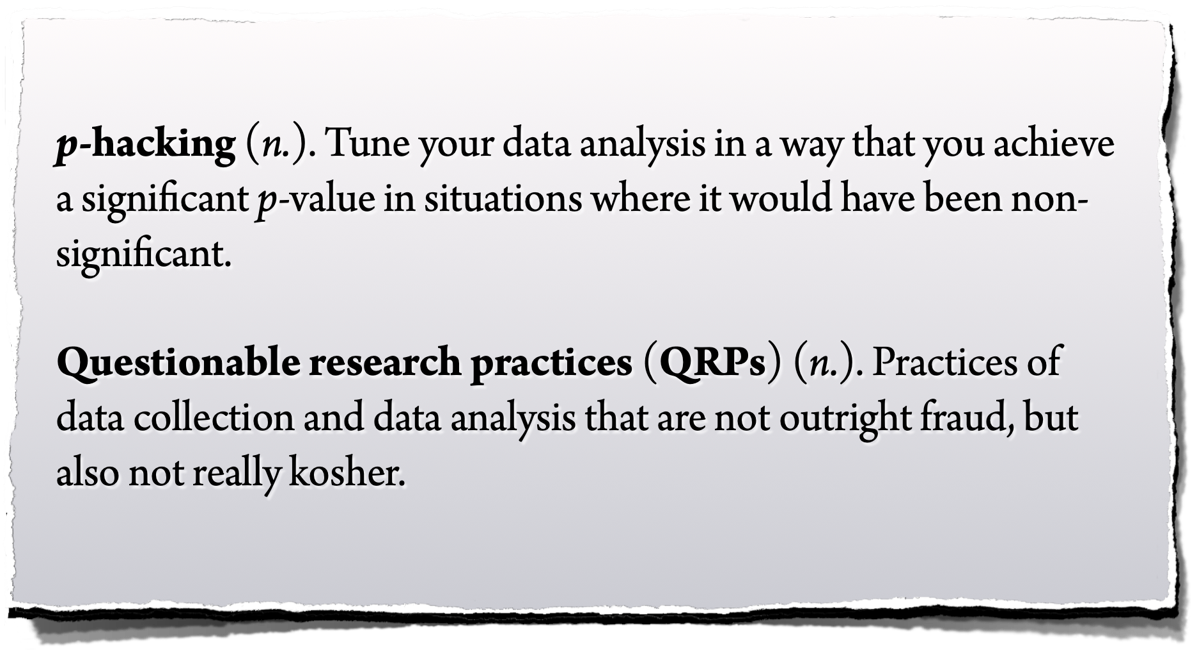
\includegraphics[width=1\linewidth,height=\textheight,keepaspectratio]{images/04_QRPs.png}
\end{center}

\textbf{Presenter Notes}: We will move to another factor which
contributes to the low reproducibility and replicability rates across
fields: accidental p-hacking. P-hacking is when researchers manipulate
their data or analyses, intentionally or not, to get a statistically
significant result (usually p \textless{} 0.05). In simple terms, it's
like trying many different tests, methods, or subsets of data until
something looks significant, and then reporting only that ``lucky''
finding. So, p-hacking is basically ``data fishing'' or
``cherry-picking'' results to make the research seem more impressive
than it really is. It is important to highlight here at this point that
p-hacking are considered questionable research practises, aka approaches
which are not yet considered fraud by the scientific community, but are
not considered ``clean'' either.

\subsection{Replicability and
reproducibility}\label{replicability-and-reproducibility-1}

\begin{tcolorbox}[enhanced jigsaw, arc=.35mm, bottomrule=.15mm, bottomtitle=1mm, breakable, colback=white, colbacktitle=quarto-callout-tip-color!10!white, colframe=quarto-callout-tip-color-frame, coltitle=black, left=2mm, leftrule=.75mm, opacityback=0, opacitybacktitle=0.6, rightrule=.15mm, title=\textcolor{quarto-callout-tip-color}{\faLightbulb}\hspace{0.5em}{Additional exercises}, titlerule=0mm, toprule=.15mm, toptitle=1mm]

Want to practice how to distinguish the two? Skip to the end of the
slides for additional exercises on replicability vs.~reproducibility.

\end{tcolorbox}

\textbf{Presenter Notes}: Want to practice how to distinguish the two?
As an extra assignment, you can skip to the end of the slides for
additional exercises on replicability vs.~reproducibility.

\textbf{Instructor Notes}: Use the extra excercises as a way to
challenge learners which may already have some prior knowledge about
these two concepts.

\subsection{Reproducibility Project:Psychology (RP:P,
2015)}\label{reproducibility-projectpsychology-rpp-2015}

\subsubsection{The first large-scale replication project in the
field}\label{the-first-large-scale-replication-project-in-the-field}

\begin{itemize}
\tightlist
\item
  \textbf{Close/exact replications} of 100 studies from 3 top journals
  from psychology; aiming for high power (larger sample sizes than
  original studies)
\item
  Different ways to judge \textbf{replication success}: evaluated based
  on effect sizes, \emph{p}-values, subjective assessment of replication
  teams
\item
  Contacted original study authors when necessary
\item
  {Note: With today's understanding of the terms, the project should
  have been called ``Replicability Project:Psychology''}
\end{itemize}

TODO: Add new slide with results. Remove the callout box.

\begin{tcolorbox}[enhanced jigsaw, arc=.35mm, bottomrule=.15mm, bottomtitle=1mm, breakable, colback=white, colbacktitle=quarto-callout-important-color!10!white, colframe=quarto-callout-important-color-frame, coltitle=black, left=2mm, leftrule=.75mm, opacityback=0, opacitybacktitle=0.6, rightrule=.15mm, title=\textcolor{quarto-callout-important-color}{\faExclamation}\hspace{0.5em}{What did they find?}, titlerule=0mm, toprule=.15mm, toptitle=1mm]

\emph{Large portion of replications produced weaker evidence for the
original findings despite using materials provided by the original
authors.}

\end{tcolorbox}

\textbf{Presenter Notes}: The Reproducibility Project by the Open
Science Collaboration (2015) involved a large-scale, collaborative
effort by over 270 researchers. They selected 100 experimental studies
published between 2008 and 2012 in three top psychology journals:
Psychological Science, Journal of Personality and Social Psychology, and
Journal of Experimental Psychology: Learning, Memory, and Cognition.

For each study, they carefully reviewed the original materials, methods,
and analyses, and often contacted the original authors for clarification
or access to materials and protocols. Each replication aimed to match
the original study's sample size, experimental design, and analysis plan
as closely as possible, while making only minimal changes when exact
materials were unavailable. The replications were preregistered to
specify hypotheses, design, and analysis before data collection,
reducing bias and ``researcher degrees of freedom.'' Data collection was
conducted independently from the original research teams, often in
multiple labs to ensure rigor. After data collection, they analyzed the
results using the same statistical methods as the original studies to
determine whether the findings could be reproduced. The project also
evaluated effect sizes, not just statistical significance, to compare
the magnitude of the original and replicated effects. \textbf{Only 39\%
of the replications produced statistically significant results, and the
median effect size in replications was about half that of the original
studies, highlighting the reproducibility challenges in psychology}.

Open Science Collaboration. (2015). Estimating the reproducibility of
psychological science. \emph{Science, 349}(6251), aac4716.

\subsection{Reproducibility Project:Psychology (RP:P,
2015)}\label{reproducibility-projectpsychology-rpp-2015-1}

\subsubsection{Results}\label{results}

\subsection{Replication rates across
disciplines}\label{replication-rates-across-disciplines}

\subsubsection{Up to 2018}\label{up-to-2018}

\begin{verbatim}
-- Attaching core tidyverse packages ------------------------ tidyverse 2.0.0 --
v dplyr     1.2.1     v readr     2.2.0
v forcats   1.0.1     v stringr   1.6.0
v lubridate 1.9.5     v tibble    3.3.1
v purrr     1.2.1     v tidyr     1.3.2
-- Conflicts ------------------------------------------ tidyverse_conflicts() --
x dplyr::filter() masks stats::filter()
x dplyr::lag()    masks stats::lag()
i Use the conflicted package (<http://conflicted.r-lib.org/>) to force all conflicts to become errors
\end{verbatim}

\pandocbounded{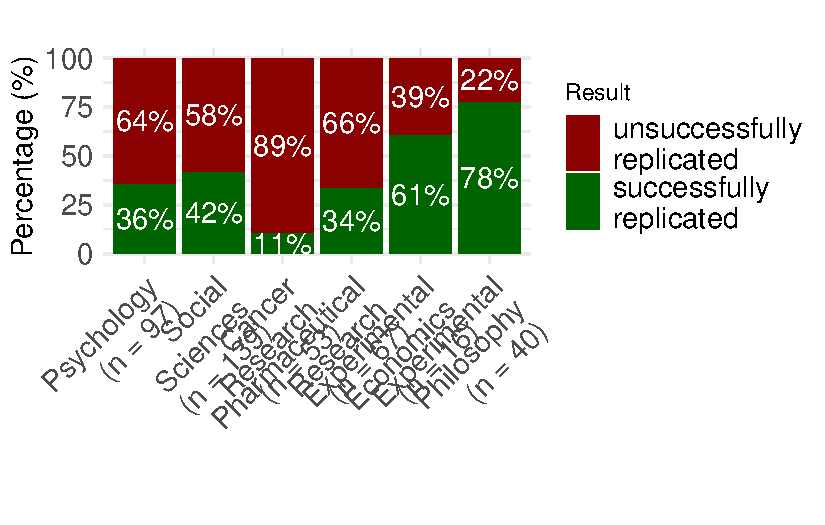
\includegraphics[keepaspectratio]{OS-M1-S1-Replicability-slides_files/figure-pdf/unnamed-chunk-2-1.pdf}}

Begley, C. G., \& Ellis, L. M. (2012); Camerer et al (2016); Chang \& Li
(2015); Cova et al.~(2018); Open Science Collaboration (2015); Social
Science: Combined sample of systematically sampled projects (RPP, SSRP,
EERP); Prinz, F., Schlange, T., \& Asadullah, K. (2011); Protzko et
al.~(2023)

\textbf{Presenter Notes}: Different studies looked at the replicability
of findings. They provide us with interesting and probably alarming
results about whether independent researchers can repeat the study using
new data and get the same overall findings or conclusions.

As you can see here, the dark red bars represents the percentage of
studies which were not successfully replicated. Psychology is quite up
there, about 64\% of all studies we conduct do not replicate. What is
equally as worrying, if not more, are that 89\% of studies from cancer
research do not replicate either. The ``best'' field really is
experimental philosophy, so from this, they have the most robust and
credible scientific approach.

\textbf{Instructor Notes}: Keep in mind that a lot of aspects of these
studies can be discussed in a critical light. Learners might point this
out. For example: Were the studies selected randomly (or did they only
select the studies that looked fishy from the start?). How do you even
measure the ``replicability``? Is simply looking for significance in the
replications study sufficient or even useful? All of these are good
points, and there is a whole emerging field that tackles these
questions. It is called meta-science, and it takes a scientific view
onto the scientific enterprise itself.

\subsection{Replication rates in the social and behavioural
sciences}\label{replication-rates-in-the-social-and-behavioural-sciences}

\textbf{Tyner et al.~(2026)}:

\begin{itemize}
\tightlist
\item
  Authors attempted \textbf{replications of 274 claims of positive
  results} from 164 quantitative papers (published between 2009 and
  2018)
\item
  \textbf{\textasciitilde55\% of positive claims replicated
  successfully}
\end{itemize}

{\def\LTcaptype{none} % do not increment counter
\begin{longtable}[]{@{}
  >{\raggedright\arraybackslash}p{(\linewidth - 4\tabcolsep) * \real{0.2250}}
  >{\raggedright\arraybackslash}p{(\linewidth - 4\tabcolsep) * \real{0.5125}}
  >{\raggedright\arraybackslash}p{(\linewidth - 4\tabcolsep) * \real{0.2625}}@{}}
\toprule\noalign{}
\begin{minipage}[b]{\linewidth}\raggedright
Discipline
\end{minipage} & \begin{minipage}[b]{\linewidth}\raggedright
Replication attempts (successful / total)
\end{minipage} & \begin{minipage}[b]{\linewidth}\raggedright
Percentage successful
\end{minipage} \\
\midrule\noalign{}
\endhead
\bottomrule\noalign{}
\endlastfoot
Business & 17 / 36 & 47.2\% \\
Economics & 10.2 / 24 & 42.5\% \\
Education & 8.2 / 13 & 63.1\% \\
Political science & 7.8 / 15 & 52.0\% \\
Psychology & 28.4 / 58 & 49.0\% \\
Sociology & 9.2 / 18 & 51.1\% \\
\end{longtable}
}

Tyner, S. K., Abatayo, A. L., Dayley, M., et al.~(2026). Investigating
the replicability of the social and behavioural sciences. Nature.
\url{https://doi.org/10.1038/s41586-025-10078-y}

\textbf{Presenter Notes}: - Authors attempted replications of 274 claims
of positive results from 164 quantitative papers (published between 2009
and 2018) in social and behavioural sciences, including psychology,
sociology, education, business, economics, and political science. -
Original materials used when available - \textasciitilde55\% of positive
claims replicated successfully

\emph{Notes:}\\
- Papers are weighted combinations of claims, accounting for multiple
claims per paper replicated in some cases.\\
- The left column shows the number of successful replications out of
total papers with replication attempts.

\subsection{Not a recent issue}\label{not-a-recent-issue}

Adapted from Dr.~Malika Ihle: \href{https://osf.io/u3znx}{https:
https://osf.io/u3znx}

\textbf{Presenter Notes}: Replication issues are not a new problem in
research; they have existed across disciplines for decades.
Historically, scientists have encountered difficulties when trying to
repeat experiments, even when methods were clearly described. This has
been seen in fields ranging from psychology and biology to medicine and
economics. What is more recent is the systematic awareness and
large-scale study of replication problems, often referred to as the
``replication crisis.'' Researchers today are documenting and
quantifying these issues, but the underlying challenges, e.g.,
methodological complexity, variability, and human error, have been part
of the research landscape for a long time.

\subsection{Why did not more studies
replicate?}\label{why-did-not-more-studies-replicate}

human error

lack of resources

cognitive bias

publication pressure

??

lack of statistical knowledge

\textbf{Presenter Notes}: The question now becomes: \textbf{Why did not
more studies replicate?} Several factors contribute to these
long-standing replication challenges. We will now have a closer look at
some of these factors.

\textbf{Instructor Notes}: Clearly state the switch into the origin for
the replication challenges and get learners curious as to why not more
studies replicated.

\section{Low power and low p(H1)}\label{low-power-and-low-ph1}

\subsection{\texorpdfstring{\faIcon{chart-bar} Live
Poll}{ Live Poll}}\label{b58fc729-690b-4000-b19f-365a4093b2ff7b7b3c2066612063686172742d6261722073697a653d3178203e7d7d-live-poll}

Given that in a given study \(p < .05\): What is the probability that a
real effect exists in the population ➙ \(p(H_1|D)\)?

\subsection{False Discovery Rate 1}\label{false-discovery-rate-1}

\pandocbounded{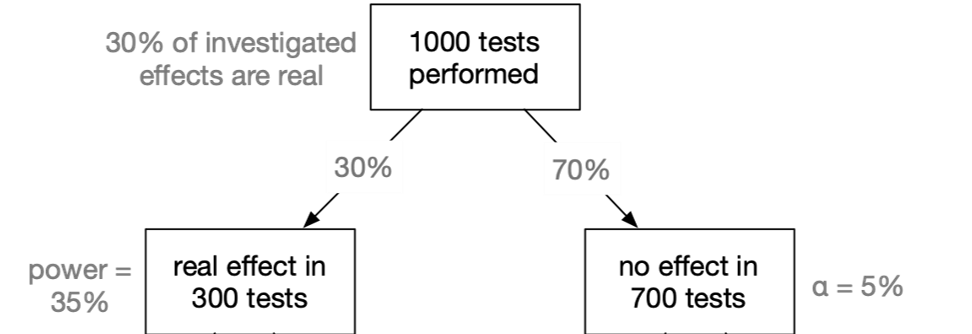
\includegraphics[keepaspectratio]{images/FDR_graph1.png}}

Nuzzo, R. (2014). Statistical errors. Nature. Colquhoun, D. (2014). An
investigation of the false discovery rate and the misinterpretation of
p-values. Royal Society Open Science, 1(3), 140216--140216.
\url{http://doi.org/10.1073/pnas.1313476110}

\subsection{False Discovery Rate 2}\label{false-discovery-rate-2}

\pandocbounded{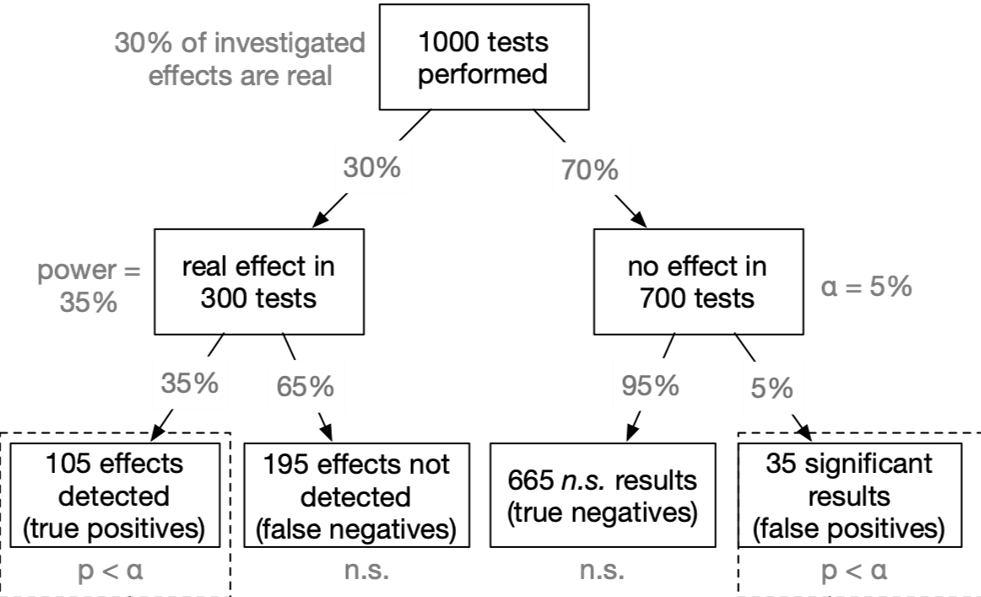
\includegraphics[keepaspectratio]{images/FDR_graph2.png}}

Nuzzo, R. (2014). Statistical errors. Nature. Colquhoun, D. (2014). An
investigation of the false discovery rate and the misinterpretation of
p-values. Royal Society Open Science, 1(3), 140216--140216.
\url{http://doi.org/10.1073/pnas.1313476110}

\subsection{False Discovery Rate 3}\label{false-discovery-rate-3}

\pandocbounded{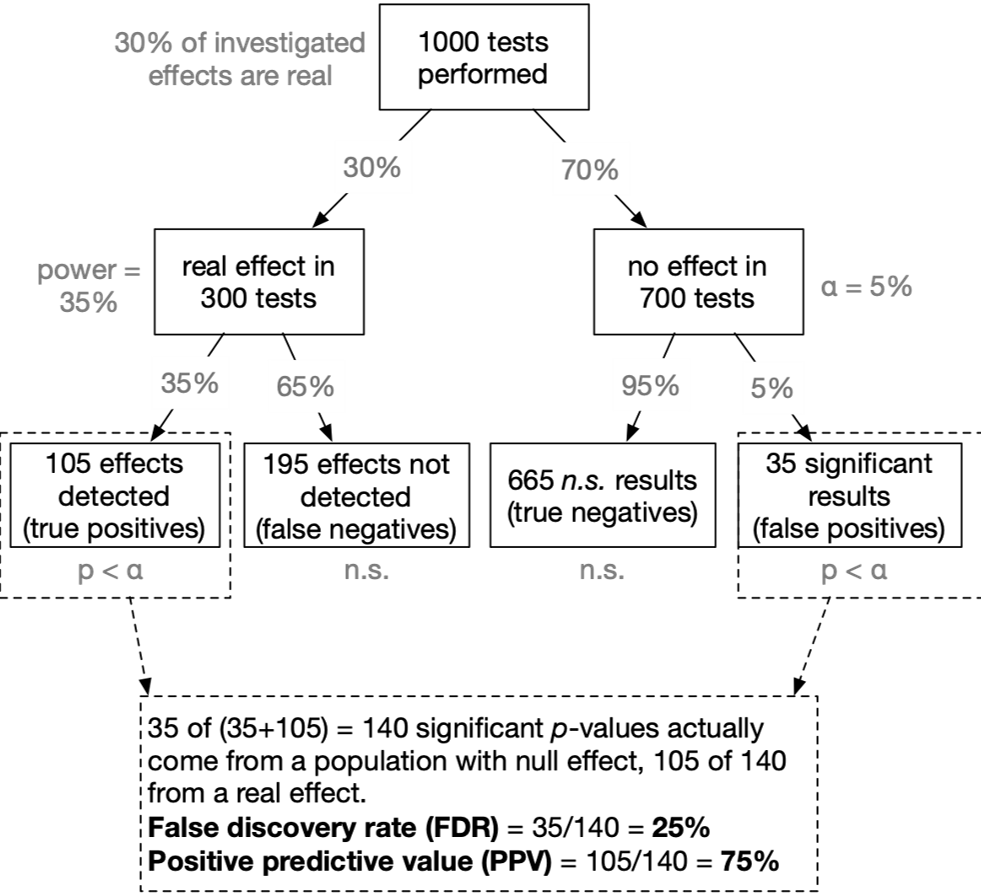
\includegraphics[keepaspectratio]{images/FDR_graph3.png}}

Nuzzo, R. (2014). Statistical errors. Nature. Colquhoun, D. (2014). An
investigation of the false discovery rate and the misinterpretation of
p-values. Royal Society Open Science, 1(3), 140216--140216.
\url{http://doi.org/10.1073/pnas.1313476110}

\subsection{Applied to neuroscience}\label{applied-to-neuroscience}

\pandocbounded{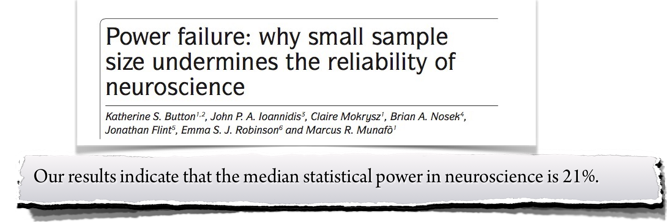
\includegraphics[keepaspectratio]{images/FDR_article1.png}}

\begin{itemize}
\tightlist
\item
  Assumed that our tested hypothesis are true in 30\% of all cases
  (which is a not too risky research scenario):

  \begin{itemize}
  \tightlist
  \item
    A typical neuroscience study must ``fail'' (\(p > \alpha\)) in 90\%
    of all cases
  \item
    In the most likely outcome of \(p > .05\), we have no idea whether
    a) the effect does not exist, or b) we simply missed the effect.
    Virtually no knowledge has been gained.
  \end{itemize}
\end{itemize}

Button, K. S., Ioannidis, J. P. A., Mokrysz, C., Nosek, B. A., Flint,
J., Robinson, E. S. J., \& Munafò, M. R. (2013). Power failure: why
small sample size undermines the reliability of neuroscience. Nat Rev
Neurosci, 14(5), 365--376. doi:10.1038/nrn3475

\subsection{The evidential strength of underpowered
studies}\label{the-evidential-strength-of-underpowered-studies}

\begin{quote}
``When a study is underpowered it most likely provides only weak
inference. Even before a single participant is assessed, it is highly
unlikely that an underpowered study provides an informative result.''

``Consequently, research unlikely to produce diagnostic outcomes is
inefficient and can even be considered unethical. Why sacrifice people's
time, animals' lives, and societies' resources on an experiment that is
highly unlikely to be informative?''
\end{quote}

Schönbrodt, F. D. \& Wagenmakers, E.-J. (2018). Bayes Factor Design
Analysis: Planning for compelling evidence. \emph{Psychonomic Bulletin
\& Review, 25}, 128-142. doi:10.3758/s13423-017-1230-y.
\href{https://osf.io/d4dcu/}{Open Access}

\subsection{Conclusion}\label{conclusion}

Given that in a given study \(p < .05\): What is the probability that a
real effect exists in the population ➙ \(p(H_1|D)\)?

\begin{itemize}
\tightlist
\item
  → In the typical situation in psychology (\(p(H_1)\) = 10\%; power =
  35\%): The probability that a significant \emph{p}-value indicates a
  true effect is only {44\%}.
\item
  Try it out yourself! \url{https://shiny.psy.lmu.de/felix/PPV}
\end{itemize}

\pandocbounded{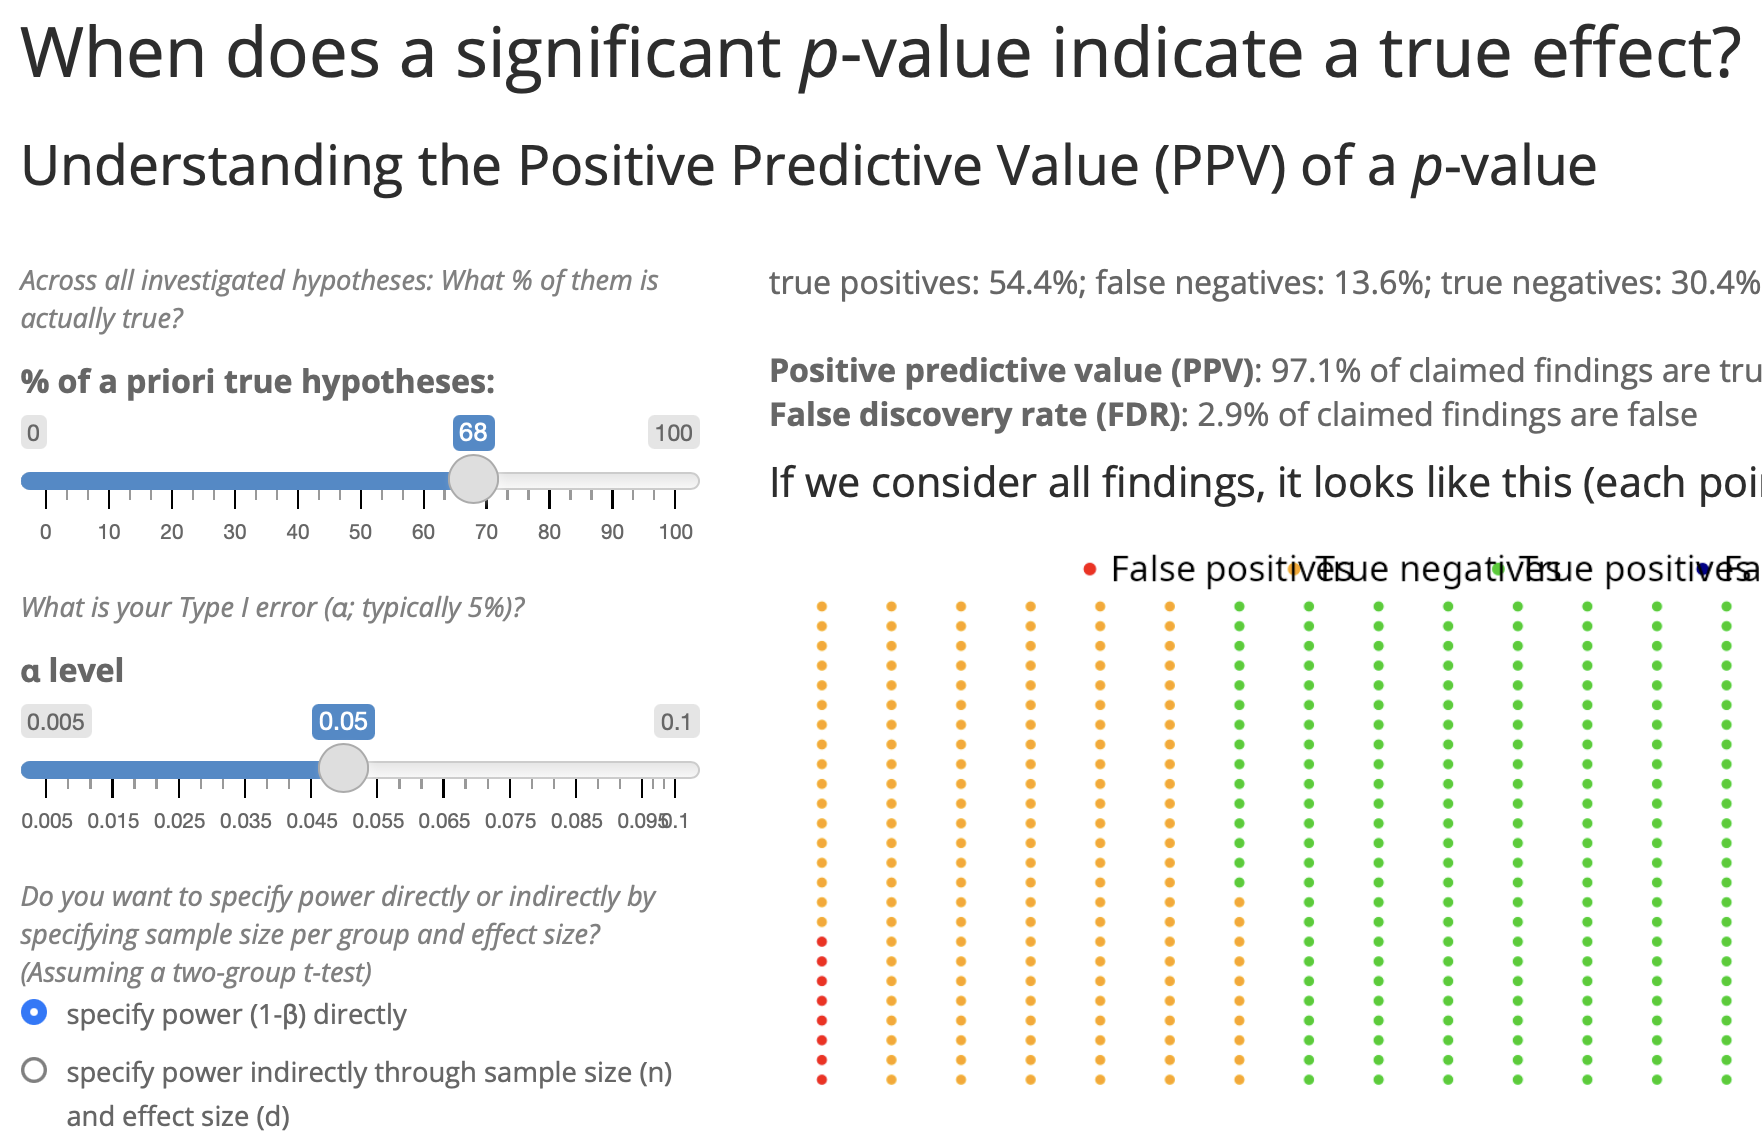
\includegraphics[keepaspectratio]{images/PPV_app.png}}

\section{Career incentives in
science}\label{career-incentives-in-science}

\subsection{How to become a professor?}\label{how-to-become-a-professor}

\begin{itemize}
\tightlist
\item
  What is the single most important thing you need to become a
  professor?
\item
  Survey among N = 1453 psychology researchers, 66\% were actually
  members of a professorship hiring committee
\end{itemize}

{\def\LTcaptype{none} % do not increment counter
\begin{longtable}[]{@{}
  >{\raggedright\arraybackslash}p{(\linewidth - 2\tabcolsep) * \real{0.9167}}
  >{\raggedright\arraybackslash}p{(\linewidth - 2\tabcolsep) * \real{0.0833}}@{}}
\toprule\noalign{}
\begin{minipage}[b]{\linewidth}\raggedright
\textbf{Actual (not desired) relevance in professorship hiring
committees}
\end{minipage} & \begin{minipage}[b]{\linewidth}\raggedright
\textbf{Rank}
\end{minipage} \\
\midrule\noalign{}
\endhead
\bottomrule\noalign{}
\endlastfoot
\textbf{Number} of peer-reviewed publications & 1 \\
Fit of research profile to the hiring department & 2 \\
Quality of research talks & 3 \\
\textbf{Number} of publications & 4 \\
Volume of acquired third party funding & 5 \\
\textbf{Number} of first authorships & 6 \\
\end{longtable}
}

Abele-Brehm, A. E., \& Bühner, M. (2016). Wer soll die Professur
bekommen? \emph{Psychologische Rundschau, 67}(4), 250--261.
\url{http://doi.org/10.1026/0033-3042/a000335}

\textbf{Presenter Notes}: There has been research which tried to look at
this element of importance of published papers. This study by
Abele-Brehm et al.~(2016) looked at criteria in the hiring process and
what the desired criteria are vs.~which criteria candidates are selected
on in real life. The growth of a scientific field depends on the people
working in it. Choosing the right people for professorships is therefore
very important. This study looks for the first time at how psychologists
view the process of hiring professors. It explores how important they
find different signs of suitability, how big the gap is between what
they want and what actually matters in these procedures, and what they
think about different ways of designing them.

A total of 3,784 members of the German Psychological Society (DGPs) were
invited to take part in an online survey, and 1,453 answered at least
some of the questions.

The take-home from this study was that among the top six criteria based
on which candidates are selected. Three are about publications and first
authorships. We have number of peer reviewed publications in the first
spot, more generally number of publications in spot 4, and the number of
first authorships, also indirectly connected to how much you published.
So, based on this, we could say great, in order to advance in academia,
all I need to do is to publish as many papers as possible, preferably
where I am the first author.

\textbf{Instructor Notes}: Highlight how quantity is rewarded of quality
of the research.

\subsection{How to become a
professor?}\label{how-to-become-a-professor-1}

\begin{tcolorbox}[enhanced jigsaw, arc=.35mm, bottomrule=.15mm, bottomtitle=1mm, breakable, colback=white, colbacktitle=quarto-callout-important-color!10!white, colframe=quarto-callout-important-color-frame, coltitle=black, left=2mm, leftrule=.75mm, opacityback=0, opacitybacktitle=0.6, rightrule=.15mm, title=\textcolor{quarto-callout-important-color}{\faExclamation}\hspace{0.5em}{Publication Pressure}, titlerule=0mm, toprule=.15mm, toptitle=1mm]

``Researchers are not rewarded for being right, but rather for
\textbf{publishing a lot}.''

\end{tcolorbox}

\begin{tcolorbox}[enhanced jigsaw, arc=.35mm, bottomrule=.15mm, bottomtitle=1mm, breakable, colback=white, colbacktitle=quarto-callout-warning-color!10!white, colframe=quarto-callout-warning-color-frame, coltitle=black, left=2mm, leftrule=.75mm, opacityback=0, opacitybacktitle=0.6, rightrule=.15mm, title=\textcolor{quarto-callout-warning-color}{\faExclamationTriangle}\hspace{0.5em}{Consequence: ``Publish or Perish'' culture}, titlerule=0mm, toprule=.15mm, toptitle=1mm]

Researchers try to \textbf{publish as much as they can} and to
outperform their peers (Schmidt et al., 2021).

\end{tcolorbox}

Nelson, Simmons, \& Simonsohn (2012); Nosek, Spies, Motyl (2012); Munafo
(2016)

\textbf{Presenter Notes}: First, we have the issue of publication
pressure. Publications are currently \emph{the} go-to measure of
academic success. Papers help researchers being considered for permanent
positions, for grants, and for becoming and remaining visible in the
respective research fields. However, a consequence of published papers
being so important is that researchers try to publish as much as they
can.

Why published papers are useful:

\begin{itemize}
\tightlist
\item
  Getting a \textbf{job} in academia
\item
  Being awarded \textbf{grant money} for your research
\item
  Being \textbf{visible} in the respective research field
\end{itemize}

\textbf{Instructor Notes}: Check if learners are aware of the
publication process in broad terms and check if they understand what
\emph{grants} means in this context.

\subsection{OK, I need a lot of publications
\ldots{}}\label{ok-i-need-a-lot-of-publications}

\subsubsection{🤔 How do I get lots of
publications?}\label{how-do-i-get-lots-of-publications}

\begin{center}
\pandocbounded{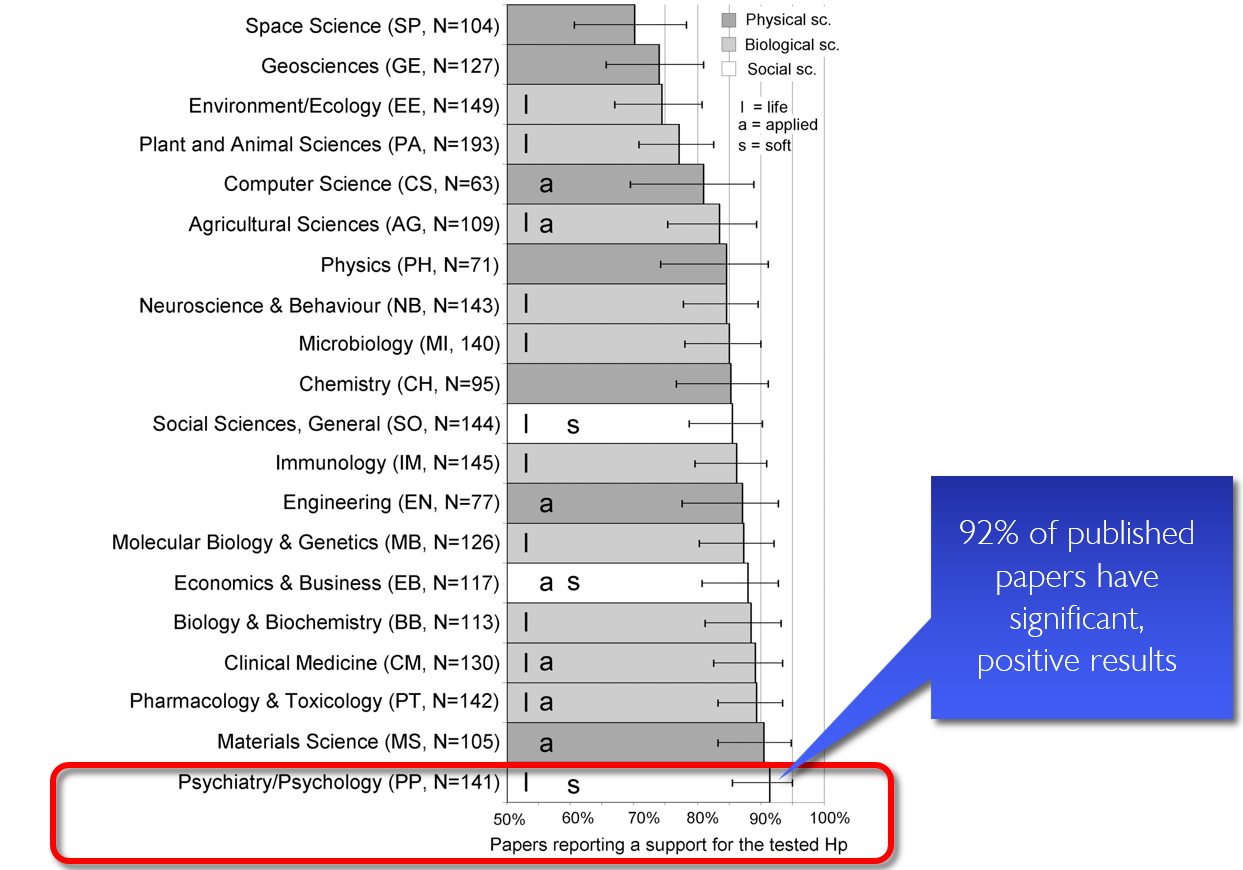
\includegraphics[keepaspectratio]{images/02_significant_results_discipline_92.png}}
\end{center}

Fanelli, D. (2010). ``Positive'' results increase down the hierarchy of
the sciences. \emph{PLOS ONE, 5}, e10068.
\url{https://doi.org/10.1371/journal.pone.0010068}

\textbf{Presenter Notes}: Following this logic, the next question
immediately becomes: \emph{well, if I need papers, how do I get papers
published?} Turns out that journals love positive results. In other
words, significant results. This study looked at published work across
all these different fields, and found that in space science, about 75\%
of published papers had significant results. In other words, 75\% of
papers were able to confirm their tested hypothesis. Great right? Then
we have statistics for many other research field, e.g., the field of
psychology or psychiatry, which can be found all the way at he bottom of
this graph. Psychology doing even better than space science, because in
their papers, 92\% of results are significant. Is that not great? 92\%
of their papers support the hypothesis researchers had generated. And
clearly what this also means is that, if I want to get published in a
psychological journal, all I need to do is bring significant, positive
results. Seems easy enough, but how do we do that?

\textbf{Instructor Notes}: Depending on your learners, highlight the
relevant field or a related field.

\subsection{Publication bias}\label{publication-bias}

``If my study \emph{works}, I can publish it. \emph{If it does not,
let's hide it the drawer.}''

\textbf{Publication bias} happens when studies with \emph{positive} or
\emph{significant} results are much more likely to be published than
studies with negative or non-significant results.

Song, F., Hooper, L., \& Loke, Y. K. (2013). Publication bias: what is
it? How do we measure it? How do we avoid it?. \emph{Open Access Journal
of Clinical Trials}, 71-81. \url{https://doi.org/10.2147/OAJCT.S34419}

\textbf{Presenter Notes}: The simplest way to obtain many papers with
positive results is to, well, publish the papers with positive results.
The logic behind it is: If my study works and the results are good
(=positive) I can publish. If not, let's pretend the study never
happened. This can be captured under the term \emph{publication bias}.
Publication bias happens when studies with positive or significant
results are much more likely to be published than studies with negative
or non-significant results.

\subsection{Example publication bias}\label{example-publication-bias}

\begin{center}
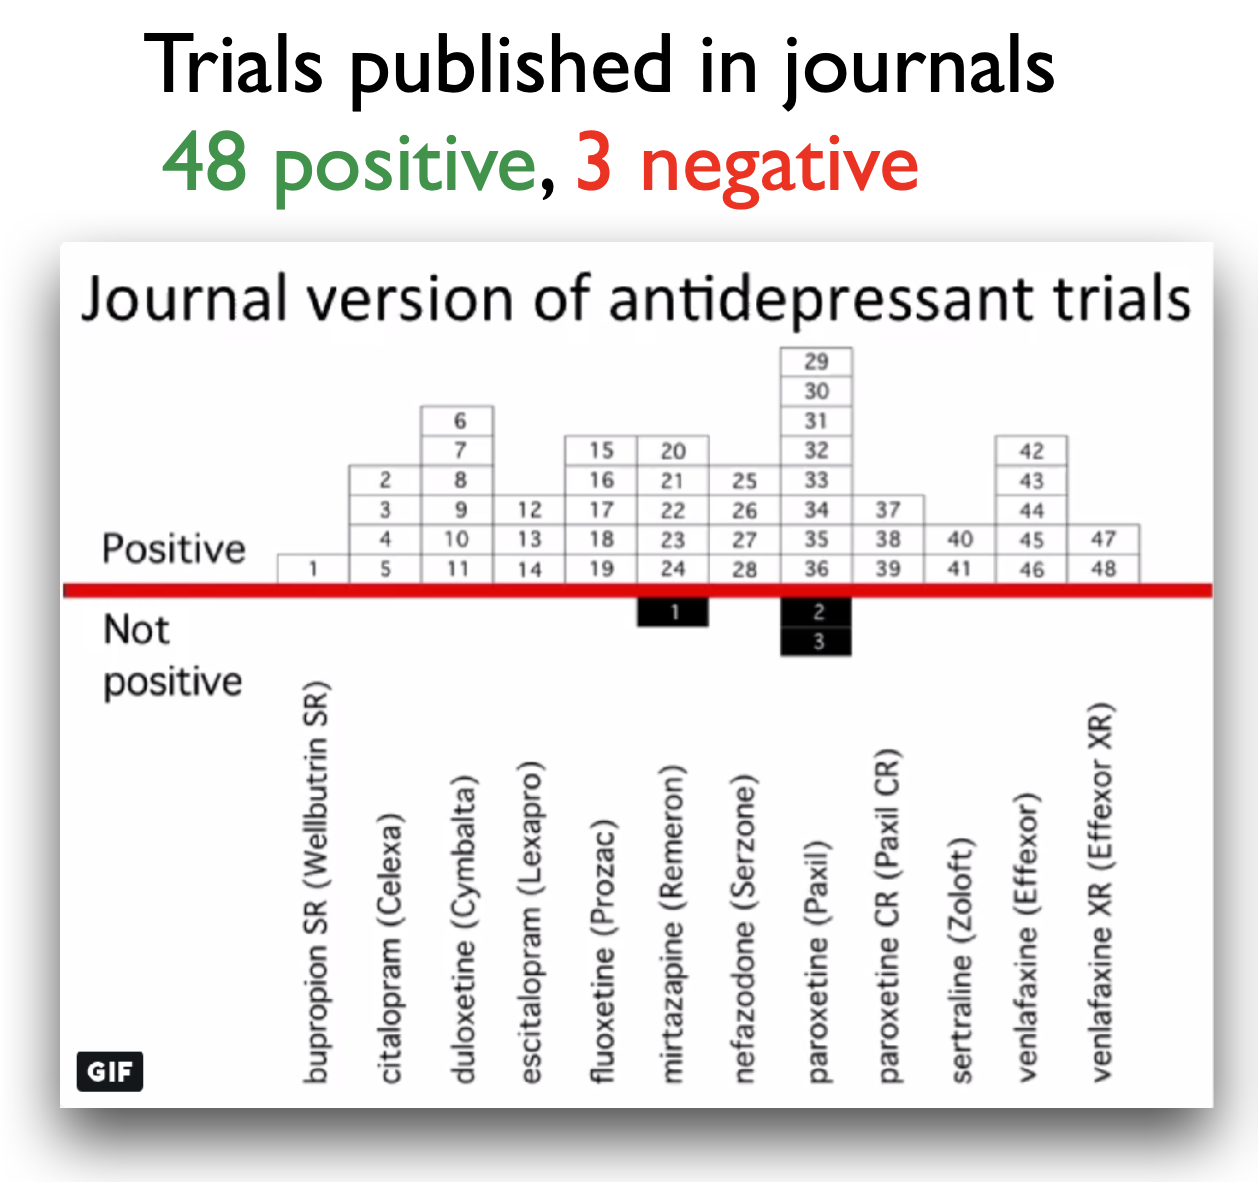
\includegraphics[width=1\linewidth,height=\textheight,keepaspectratio]{images/Turner_Study_Publication_Bias_1.png}
\end{center}

\begin{center}
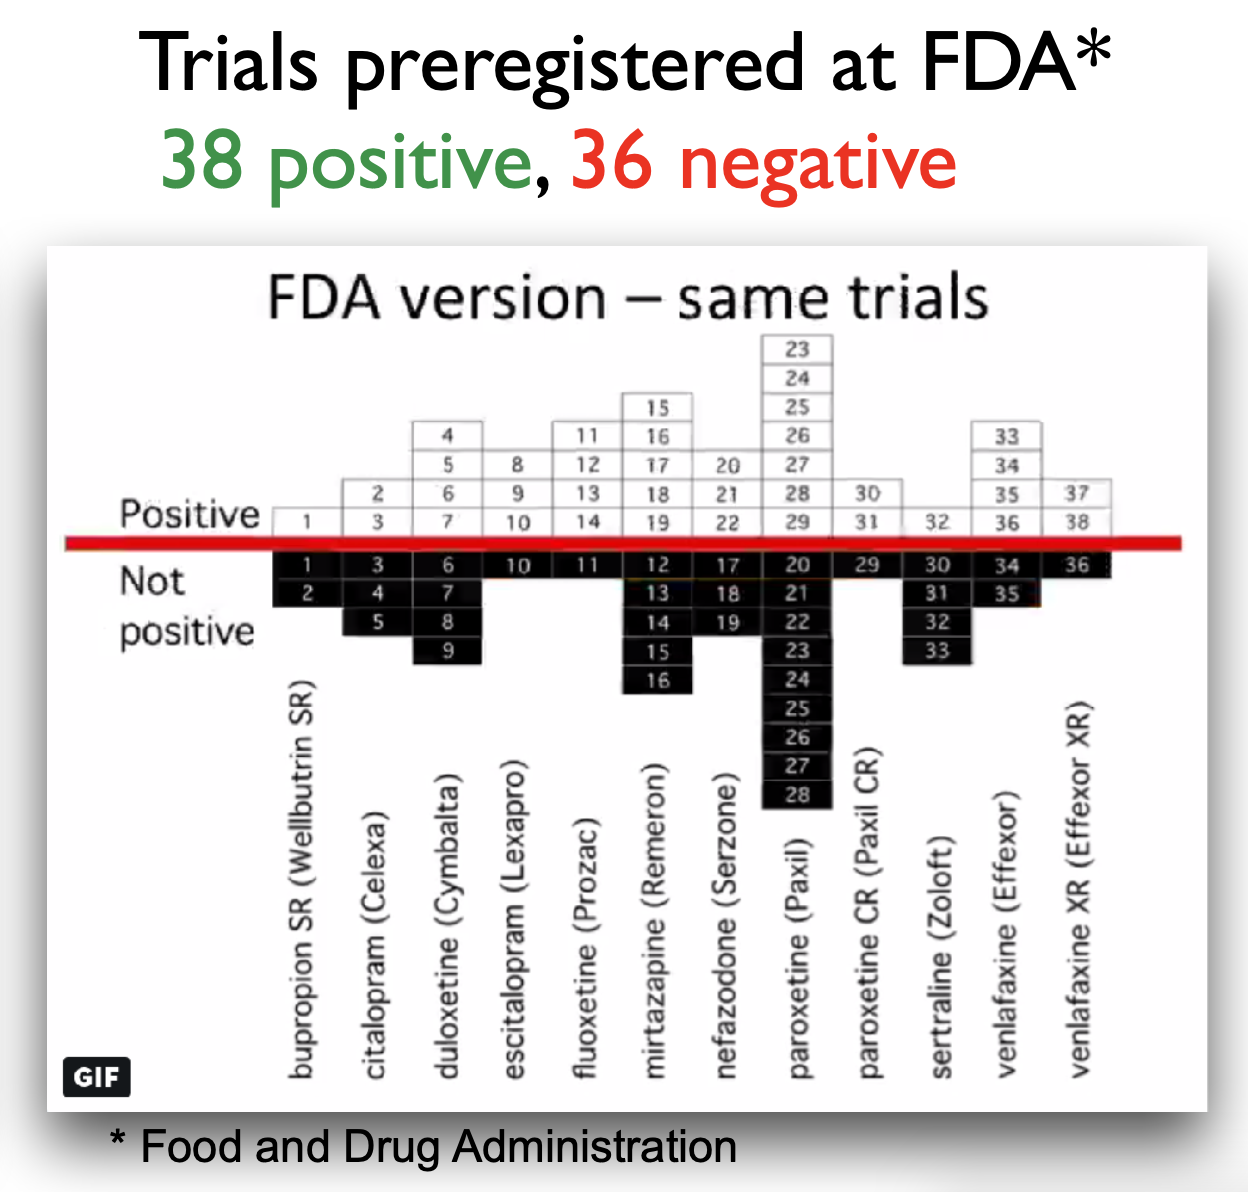
\includegraphics[width=1\linewidth,height=\textheight,keepaspectratio]{images/Turner_Study_Publication_Bias_2.png}
\end{center}

Turner, E. H., Matthews, A. M., Linardatos, E., Tell, R. A., \&
Rosenthal, R. (2008). Selective publication of antidepressant trials and
its influence on apparent efficacy. \emph{New England Journal of
Medicine, 358}(3), 252-260. \url{https://doi.org/10.1056/NEJMsa065779}

\textbf{Presenter Notes}: Turner and colleagues (2008) studied how
selective publication bias affects research on antidepressant drugs.
They compared antidepressant trials registered with the FDA to what was
actually published in journals. They found that studies with positive
results were much more likely to be published than those with negative
or uncertain results. This made antidepressants seem more effective than
they really were. Specifically, their analysis showed that about half of
all FDA-registered trials did not show clear benefits, but almost all
positive studies were published. In contrast, most negative studies were
either not published at all or were written in a way that made the
results look better than they were. This bias gave an inflated view of
how well antidepressants work.

\textbf{Instructor Notes}: Additional details about the study and the
conclusions: In this study, the authors obtained the archive of clinical
trials for 12 antidepressant drugs submitted the the US Food and Drug
Administration (FDA). In total, the trials involved more than 12000
patients. They performed a systematic search to identify which of these
trials had been published in the literature. For those that were
published, the compared the published versions and results with the
versions and results in the FDA documentation. There were 74
FDA-registered trials. Of those, 38 trials showed postive effects of
antidepressant drugs, 36 showed negative effects of antidepressant
drugs. This is a 51\% - 49\% split of results: about half of the
FDA-registered trials showed a positive effect of antidepressant drugs,
the other half showed a negative effect of antidepressant drugs. 37 of
the 38 trials that showed positive effects were published in the
literature, basically all of them except 1 trial. However, of the 36
trials that showed negative or no effects of antidepressant drugs, only
3 were published that included those exact findings. 22 of the 36 trials
were not published at all, and the remaining 11 trials were published
with the outcomes reframed in a more positive way. In the literature, in
the end, we ended up with a total of 51 trials being published, 48 of
which showed positive effects of antidepressant drugs on depression.
That is 94\% of this sample of papers. Only 6\% (3 papers) showed a
negative effect of antidepressant drugs on depression. As a consequence,
those of us searching the literature for these papers, will get a
distorted via of the effectiveness of antidepressants. Therefore, the
authors were able to show a substantial publication bias in the
antidepressant trial literature.

\subsection{More than just publication
bias}\label{more-than-just-publication-bias}

\begin{enumerate}
\def\labelenumi{(\alph{enumi})}
\tightlist
\item
  All conducted studies
\item
  \textbf{Study publication bias}: non-publication of an entire study
\item
  \textbf{Outcome reporting bias}: non-publication of negative outcomes
  within a published article or switching the status of
  (non-significant) primary and (significant) secondary outcomes
\item
  \textbf{Spin}: authors conclude that the treatment is effective
  despite non-significant results on the primary outcome
\item
  \textbf{Citation bias}: Studies with positive results receive more
  citations than negative studies
\end{enumerate}

De Vries, Y. A., Roest, A. M., de Jonge, P., Cuijpers, P., Munafò, M.
R., \& Bastiaansen, J. A. (2018). The cumulative effect of reporting and
citation biases on the apparent efficacy of treatments: the case of
depression. \emph{Psychological Medicine, 48}(15), 2453--2455.
\url{https://doi.org/10.1017/S0033291718001873}

\textbf{Presenter Notes}: This paper by de Vries and colleagues (2018)
showed that there might be more than ``just'' publication bias at play.
What we are looking at here in this graph is the following:

\begin{enumerate}
\def\labelenumi{\alph{enumi})}
\item
  The authors assembled a cohort of 105 randomised controlled trials
  (RCTs) of antidepressant treatments for depression, drawn from the
  Food and Drug Administration (FDA) registration/trial-submission
  database (74 trials from an earlier study plus 31 newer ones). They
  found that of these 105 trials: 53 (50\%) trials were showed
  statistically significant positive effects of antidepressant
  treatments and 52 (50\%) trials did not show a statistically positive
  effect of antidepressant treatment.
\item
  They found that all of the trials with positive results, so a totlal
  of 53 trials, we then published. However, as you can see here, only
  about half of the trials with negative results were published. This
  represents the classical study publication bias we discussed
  previously.
\item
  Of the trials that were published, something interesting happened to
  the ones with negative results. Upon publishing, some trials were
  published in a way that made them appear positive by omitting
  unfavourable outcomes, or by switching the designation of primary
  versus secondary outcomes.
\item
  You can see now how the number of published trials with negative
  outcomes are slowly decreasing. The next reduction of negative
  published trials comes from what we call spin. For some trials, even
  when primary outcomes are non-significant, authors may write the
  abstract in a positive way. In other words, authors interpret
  statistically negative results in a more positive light than supported
  by the data.
\item
  Finally, we also have citation bias, which is simply the phenomenon
  that studies with positive results get cited more, as you can see here
  by these different circles. The ones that come out very strongly are
  the ones that get cited more often, and you can see that all of those
  are the trials with positive results. In contrast, the ones with
  ``spin results'' or negative results, get cited much less often. In
  the study's cohort, after accounting for publication and
  outcome-reporting biases, the remaining published positive studies
  tended to have higher visibility (more citations) than the published
  negative ones. The authors also note that positive trials were
  published in journals with higher median impact factor than negative
  ones (for antidepressants: 3.5 vs 2.4), which likely contributes to
  higher citations and visibility.
\end{enumerate}

\textbf{Instructor Notes}: This is a complex figure, take your time with
walking learners through this step-by-step.

\subsection{Confirmation Bias}\label{confirmation-bias}

\subsubsection{a.k.a. ``Thought so already''
bias}\label{a.k.a.-thought-so-already-bias}

\begin{center}
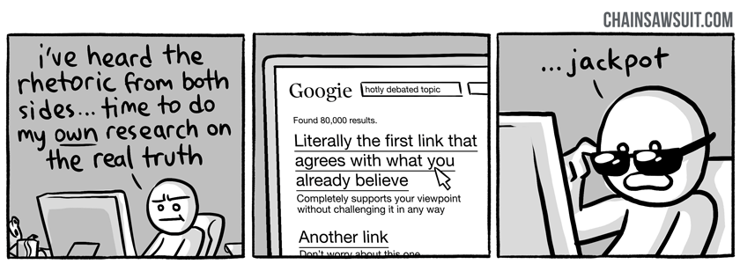
\includegraphics[width=1\linewidth,height=\textheight,keepaspectratio]{images/14_cognitive_bias.png}
\end{center}

\textbf{Presenter Notes}: We are humans. And as humans, we often fall
victims to our own inherent biases, sometimes or quite often without us
noticing. Sometimes we cannot help but to feel like we just unlocked
evidence or proof for something that we suspected all along. And it can
be that it is true, or just that we stopped looking for more evidence
and arguments as soon as we found the evidence that corresponded to our
way of thinking. This is called the \textbf{confirmation bias}.
Confirmation bias refers to the tendency to look for, interpret, or
remember information in a way that confirms your pre-existing beliefs or
expectations, while ignoring or downplaying evidence that contradicts
them. In research, this can lead to selective attention to data, skewed
analyses, or overconfident conclusions. For example; imagine a
researcher believes that a new study technique helps students perform
better. While analyzing results, they might focus on the small group of
students who improved and overlook those whose performance stayed the
same or worsened. Even unintentionally, this bias can make the findings
seem stronger or more conclusive than they really are.

\subsection{Hinsight Bias}\label{hinsight-bias}

\subsubsection{a.k.a. ``I knew it'' bias}\label{a.k.a.-i-knew-it-bias}

\begin{center}
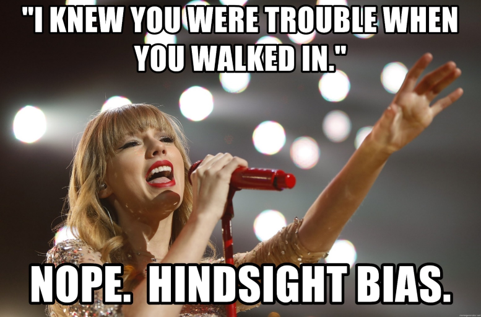
\includegraphics[width=7\linewidth,height=\textheight,keepaspectratio]{images/hindsight-bias.png}
\end{center}

\begin{itemize}
\tightlist
\item
  The tendency to believe, after seeing the results of a study, that the
  outcome was obvious or predictable all along, even if it was not.
\end{itemize}

\textbf{Presenter Notes}: Another bias we are unconsciously struggling
with in the research process is this \textbf{hindsight bias}. It is the
tendency to believe, after seeing the results of a study, that the
outcome was obvious or predictable all along, even if it was not. For
example: Imagine a study finds that people who exercise regularly have
lower stress levels. After seeing the results, a researcher might think,
``Of course, I knew exercise would reduce stress!'' Even though before
the study, this connection was not at all certain. Hindsight bias can
make results seem more predictable than they really were, which can lead
researchers or readers to overestimate the certainty of findings or
ignore alternative explanations.

\subsection{Practical exercise 4}\label{practical-exercise-4}

\textbf{Task}: Match the bias to its description.

{\def\LTcaptype{none} % do not increment counter
\begin{longtable}[]{@{}
  >{\raggedright\arraybackslash}p{(\linewidth - 2\tabcolsep) * \real{0.4138}}
  >{\raggedright\arraybackslash}p{(\linewidth - 2\tabcolsep) * \real{0.5862}}@{}}
\toprule\noalign{}
\begin{minipage}[b]{\linewidth}\raggedright
\textbf{Bias}
\end{minipage} & \begin{minipage}[b]{\linewidth}\raggedright
\textbf{Description}
\end{minipage} \\
\midrule\noalign{}
\endhead
\bottomrule\noalign{}
\endlastfoot
\textbf{1.} Confirmation bias & \textbf{A.} Non-publication of negative
outcomes within a paper, or switching non-significant primary outcomes
with significant secondary ones. \\
\textbf{2.} Spin & \textbf{B.} Studies with positive results receive
more citations than negative studies. \\
\textbf{3.} Study publication bias & \textbf{C.} After learning the
outcome, believing ``I knew it all along.'' \\
\textbf{4.} Hindsight bias & \textbf{D.} Non-publication of an entire
study (e.g., trials with null results never submitted). \\
\textbf{5.} Outcome reporting bias & \textbf{E.} Tendency to seek or
interpret information in ways that confirm existing beliefs. \\
\textbf{6.} Citation bias & \textbf{F.} Authors conclude the treatment
is effective despite non-significant primary outcomes. \\
\end{longtable}
}

\textbf{Presenter Notes}: Time for another exercises, To consolidate the
different biases a little, let's atry and match the biases to their
respective descriptions. Then we discuss in the group.

\textbf{Instructor Notes}: Solutions: 1E, 2F, 3D, 4C, 5A, 6B. Give about
5 minutes for this exercise and 2 minutes for discussing the correct
results.

\section{Pre-break survey}\label{pre-break-survey}

\textbf{Presenter Notes}: Before we head into a short break, let us
revise some concepts again and see where we are at.

\textbf{Instructor Notes}:

\begin{itemize}
\item
  \textbf{Aim}: This pre-break survey serves to examine students'
  current understanding of key concepts of the submodule
\item
  Use free survey software such as particify or formR to establish the
  following questions (shown on separate slides)
\end{itemize}

\subsection{Pre-break survey}\label{pre-break-survey-1}

\textbf{Based on what you learnt so far, how would you \emph{now} rate
your trust in published scientific findings on a scale from 1 - 5? (1 =
not trusting any of the findings, 2 = trusting only some findings, 3 =
trusting about half of the findings, 4 = trusting the majority of the
findings, 5 = trusting all findings)}

\begin{enumerate}
\def\labelenumi{\alph{enumi}.}
\item
  1
\item
  2
\item
  3
\item
  4
\item
  5
\end{enumerate}

\textbf{Presenter Notes}: Coming back to the question from the
beginning, what is your current trust in research with this information
from the slides?

\subsection{Pre-break survey}\label{pre-break-survey-2}

\textbf{What does \emph{replicability} in research mean?}

\begin{enumerate}
\def\labelenumi{\alph{enumi}.}
\item
  Obtaining the same results using the original dataset and code
\item
  Obtaining consistent results when a new study collects new data using
  the same methods
\item
  Publishing results in more than one journal
\item
  Repeating the statistical analysis multiple times
\end{enumerate}

\textbf{Instructor Notes}: The correct answer is b.

\subsection{Pre-break survey}\label{pre-break-survey-3}

\textbf{What is \emph{publication bias} in research?}

\begin{enumerate}
\def\labelenumi{\alph{enumi}.}
\item
  The tendency for journals to publish studies only from well-known
  researchers
\item
  The requirement that all published studies must be peer-reviewed
\item
  The practice of publishing the same study in multiple journals
\item
  The tendency for studies with positive results to be published more
  often than studies with non-significant or negative results
\end{enumerate}

\textbf{Instructor Notes}: The correct answer is d.~

\section{Break! 15 minutes}\label{break-15-minutes}

\subsection{Post-break survey
discussion}\label{post-break-survey-discussion}

What do we see in the results?

\textbf{Presenter Notes}: Add.

\textbf{Instructor Notes}:

\begin{itemize}
\item
  \textbf{Aim}: To clarify concepts and aspects that are not yet
  understood
\item
  Highlight specific answers given during the survey
\end{itemize}

\section{p-hacking and other problems
\ldots{}}\label{p-hacking-and-other-problems}

\begin{tcolorbox}[enhanced jigsaw, arc=.35mm, bottomrule=.15mm, bottomtitle=1mm, breakable, colback=white, colbacktitle=quarto-callout-warning-color!10!white, colframe=quarto-callout-warning-color-frame, coltitle=black, left=2mm, leftrule=.75mm, opacityback=0, opacitybacktitle=0.6, rightrule=.15mm, title=\textcolor{quarto-callout-warning-color}{\faExclamationTriangle}\hspace{0.5em}{Warning}, titlerule=0mm, toprule=.15mm, toptitle=1mm]

Do \textbf{not} try the following at home.

\end{tcolorbox}

\subsection{\texorpdfstring{``Hack'' 1: Add \emph{lots} of outcome
variables}{``Hack'' 1: Add lots of outcome variables}}\label{hack-1-add-lots-of-outcome-variables}

\begin{itemize}
\item
  For \textbf{two outcome variables}: False positive rate increases from
  5\% to \textbf{9.5\%}
\item
  For \textbf{five outcome variables} (and one-sided testing): False
  positive rate increases from 5\% to \textbf{41\%}
\end{itemize}

\begin{center}
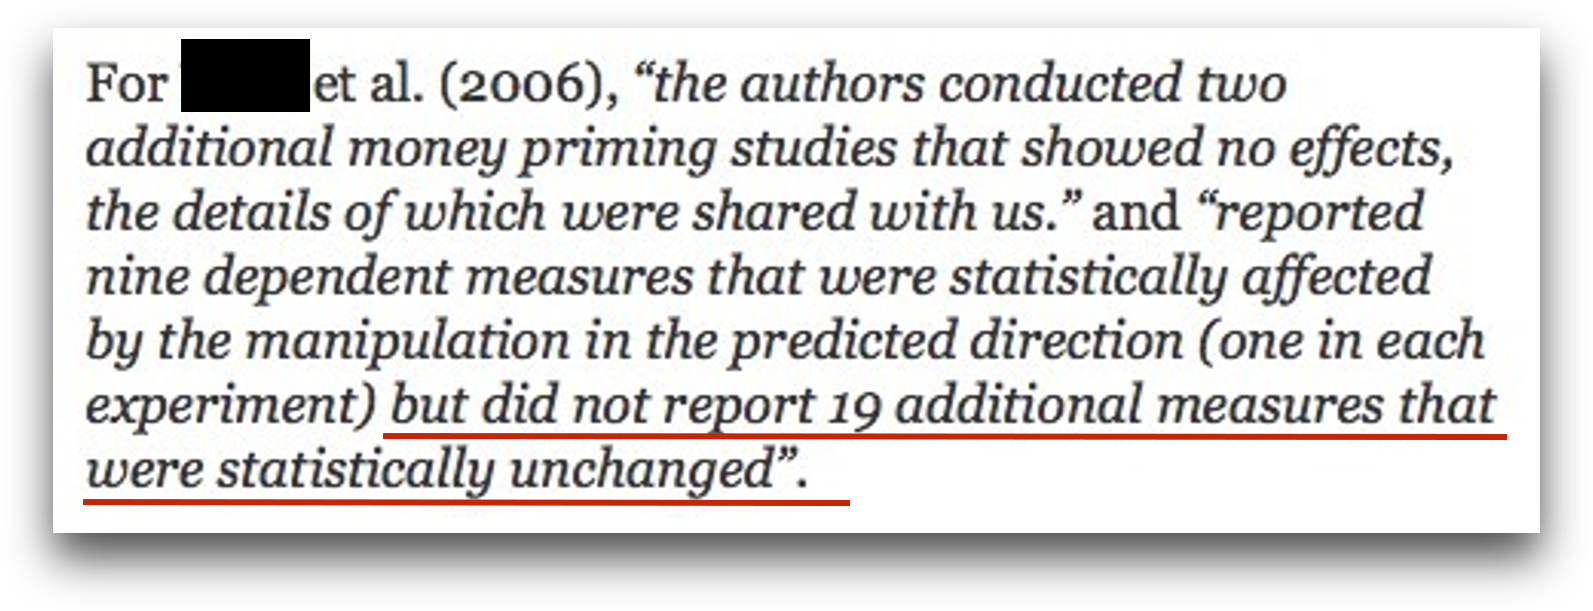
\includegraphics[width=1\linewidth,height=\textheight,keepaspectratio]{images/05_Outcome_Switching.png}
\end{center}

\textbf{Presenter Notes}: Let us say you designed an experiment,
generated a hypothesis and collected some data. Now you are analysising
your data and are running a statistical test. When you run a statistical
test, you're checking whether your data could have happened just by
random chance. If the p-value, which is the probability of getting your
result if there's really no effect, is less than 0.05, you say the
result is ``statistically significant.'' That means there's less than a
5\% chance that the result happened by luck, assuming the null
hypothesis is true. With a p-value below 0.05, you are saying, ``I'm
fairly confident this effect is real. There's only about a 5\% or a 1 in
20 chance that I incorrectly conclude that an effect or a difference
between two conditions exists''. In other words, it is the probability
that I find a false positive.

However, when you run multiple tests, each one carries its own 5\%
chance of producing a false positive, and these chances add up. As a
result, the overall likelihood of finding at least one false positive
across all tests, known as the family-wise error rate, becomes much
higher than 5\%. For example, if you test two outcome variables, each at
the 5\% significance level, the combined chance that at least one result
is a false positive increases to about 9.5\%.

If you test five outcome variables, that overall false positive rate can
rise dramatically, up to around 41\% for one-sided tests. In simple
terms, the more outcomes you test, the greater your risk of finding a
``significant'' result purely by chance. So your chance of a false
positive results is extremely high. I would therefore recommend
including as many outcome variables as possible, you are sure to find a
significant results for at least one of them.

\textbf{Instructor Notes}: Additional information for students: To
reduce the false-positive rate, researchers often apply corrections,
such as the Bonferroni adjustment, to keep the overall false positive
rate close to the intended 5\%.

\subsection{``Hack'' 2: Run as many comparisons as
possible}\label{hack-2-run-as-many-comparisons-as-possible}

\begin{itemize}
\tightlist
\item
  Run as many different comparisons on \textbf{different outcomes,
  subgroups, time windows} etc. as you can
\item
  \textbf{Only} report the comparisons that produced a statistically
  significant result
\end{itemize}

O'Boyle, E. H., Banks, G. C., \& Gonzalez-Mulé, E. (2017). The Chrysalis
Effect: How ugly initial results metamorphosize into beautiful articles.
\emph{Journal of Management, 43}(2), 376--399.
\url{https://doi.org/10.1177/0149206314527133}

\textbf{Presenter Notes}: When you have more outcome variables, this
often also means that you can run more statistical tests. Each time you
try another independent test at α = 0.05 you have a 5\% chance of a Type
I error for that test. If you perform many uncorrected tests, the chance
that at least one will be (falsely) significant rises quickly. For
example, doing 20 independent tests at α = 0.05 gives a probability of
at least one false positive of1 − (1 − 0.05)²⁰ = 1 − 0.95²⁰ ≈ 0.6415
(≈64\%). Therefore, the trick here is to just run as many comparisons as
possible on different groups, different time windows, different
subsections of your data, you will be guaranteed to find significant
results. Then, of course, only report those comparisons that produced
the significant result. Just run many more statistical tests and report
only the ones you like. Easy, right?

\subsection{``Hack'' 2: Run as many comparisons as
possible}\label{hack-2-run-as-many-comparisons-as-possible-1}

\subsubsection{Example: Subgroup
Analyses}\label{example-subgroup-analyses}

Research question: Do aggressive primes trigger aggressive behavior?

\begin{quote}
``A second study in Turner, Layton, and Simons (1975) collects a larger
sample of men and women driving vehicles of all years. The design was a
2 (Rifle: present, absent) × 2 (Bumper Sticker:''Vengeance'', absent)
design with 200 subjects.''
\end{quote}

➙ presumably, no effect \ldots{} (yet! Do not give up so easily)

Cited from Joe Hilgard's excellent
\href{http://crystalprisonzone.blogspot.com/2016/03/the-weapons-priming-effect.html}{blog
post} on the Weapon Priming Effect; Turner et al.~(1975). Naturalistic
studies of aggressive behavior: aggressive stimuli, victim visibility,
and horn honking. JPSP, 31(6), 1098--1107.

\subsection{``Hack'' 2: Run as many comparisons as
possible}\label{hack-2-run-as-many-comparisons-as-possible-2}

\subsubsection{Example: Subgroup
Analyses}\label{example-subgroup-analyses-1}

\begin{quote}
``They divide this further by driver's sex and by a median split on
vehicle year. They find that the Rifle/Vengeance condition increased
honking relative to the other three, \textbf{but only among
newer-vehicle male drivers}, F(1, 129) = 4.03, {\emph{p} = .047}. But
then they report that the Rifle/Vengeance condition decreased honking
among older-vehicle male drivers, F(1, 129) = 5.23, {\emph{p} = .024}!
No results were found among female drivers.''
\end{quote}

Cited from Joe Hilgard's excellent
\href{http://crystalprisonzone.blogspot.com/2016/03/the-weapons-priming-effect.html}{blog
post} on the Weapon Priming Effect; Turner et al.~(1975). Naturalistic
studies of aggressive behavior: aggressive stimuli, victim visibility,
and horn honking. JPSP, 31(6), 1098--1107.

\subsection{``Hack'' 3: Optional
stopping}\label{hack-3-optional-stopping}

\begin{itemize}
\tightlist
\item
  Scenario: You collect a sample of \emph{n}=60 and obtained a
  \emph{p}-value of .07.
\item
  ``Trending towards significance''! \textbf{What is your intuition how
  to proceed?}
\end{itemize}

\pandocbounded{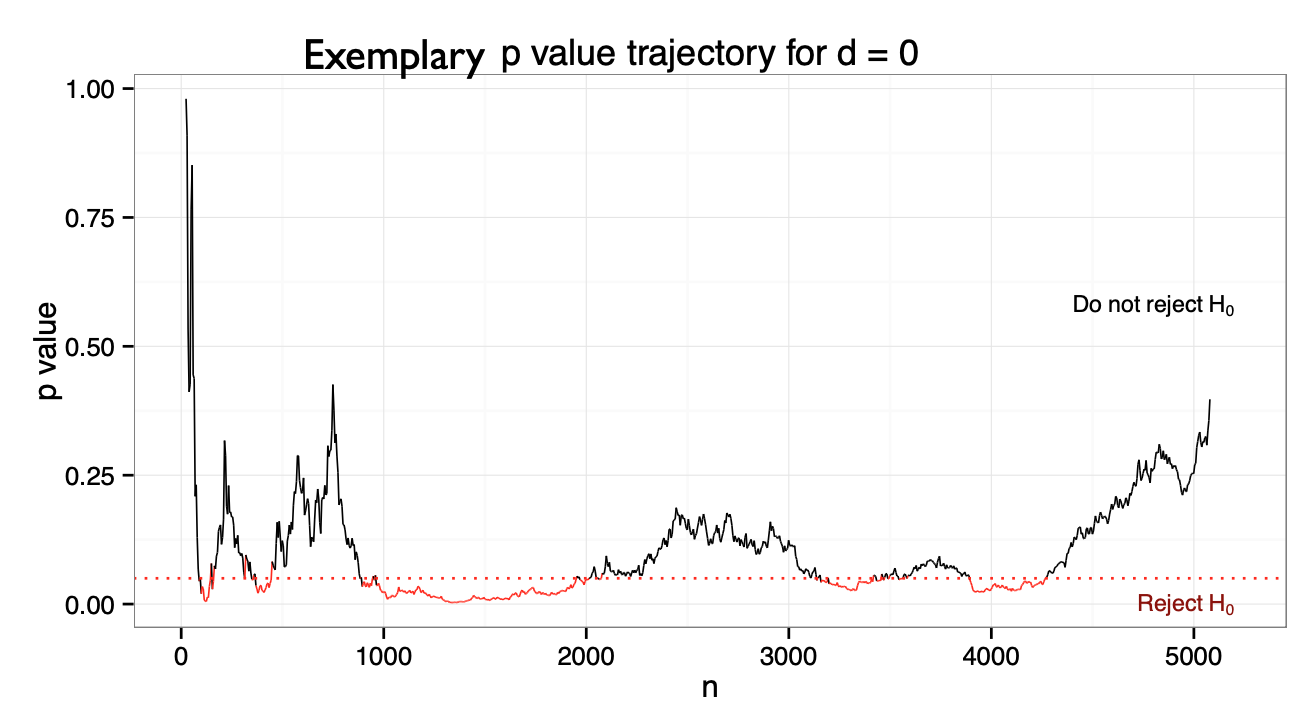
\includegraphics[keepaspectratio]{images/p-value-trajectory.png}}

\textbf{Presenter Notes}: Another p-hacking strategy is called peeking
or \textbf{optional stopping}. In other words, you start doing your
analysis already before all data have been collected and perform
multiple interim analyses ``just to have a look''. With every interim
analysis, you are, of course, increasing your chances of finding a false
positive, or, what you would consider a ``true'' significant effect that
is, unfortunately not true at all.

You do not have to take my word for it that this practice can increase
the false positive rates, but there have been some people who looked at
this. Their work demonstrated that when researchers test interim results
multiple times and stop data collection once a significant result
appears, the false positive rate does not stay at 5\%. Instead, this
rate increases exponentially with each additional interim analysis. Even
a modest number of repeated tests can double or triple the chance of
declaring a false positive. This inflation occurs because each interim
look introduces another opportunity for a random fluctuation to cross
the significance threshold. In other words, you can move from a 5\%
chance of incorrectly concluding that there is an effect to an 11\%
chance with only one additional analyses.

So, the moral of the story here is that you need to just do as many
interim analyses as possible before you finish your data collection, and
I guarantee you will obtain a significant results at some point. When
you do, of course ``there is no point in sticking to your original plan
of minimum sample size, so to not waste time, you should also stop data
collection immediately''.

\textbf{Instructor Notes}: Explicitly highlight the sarcastic aspect of
this slide, since there are large cultural differences in whether and
how sarcasm is perceived as a linguistic cue and processed. Reframe this
slide if you have the impression that the audience will not benefit from
sarcasm.

\subsection{``Hack'' 3: Optional
stopping}\label{hack-3-optional-stopping-1}

\begin{itemize}
\tightlist
\item
  Optional stopping: Collect an initial sample, analyze the results, add
  participants if the results are not significant
\item
  But under \(H_0\), the \emph{p}-value is a random walk between 0 and
  1, fluctuating forever.
\item
  Eventually, it will ``dip'' below the critical threshold
\item
  The false positive rate depends on the number of optional sample size
  increases:

  \begin{itemize}
  \tightlist
  \item
    One analysis: α = 5\%
  \item
    Two analyses: α = 11\%
  \item
    But with enough increases can be pushed to 100\%!
  \end{itemize}
\end{itemize}

Armitage, P., McPherson, C. K., \& Rowe, B. C. (1969). Repeated
significance tests on accumulating data. \emph{Journal of the Royal
Statistical Society. Series A (General), 132}, 235--244.

\subsection{``Hack'' 4: Drop participants you do not
like}\label{hack-4-drop-participants-you-do-not-like}

\begin{itemize}
\tightlist
\item
  Selectively \textbf{exclude data/ outliers} after seeing the results
  until the results are satisfying (\emph{aka until significance has
  been reached})
\end{itemize}

\textbf{Presenter Notes}: Another common form of p-hacking happens when
researchers selectively remove outliers or participants from their
dataset to make their results look more significant. In simple terms, an
outlier is a data point that looks very different from the rest. This is
maybe a participant who scored unusually high or low compared to the
rest of the participants. Sometimes, removing outliers is justified, for
example, if there was a clear measurement error. But in order to obtain
significant results, you can also perform a first analysis, evaluate
your p-values and think about excluding those participants that are just
really, really biasing your data. Of course, this practice increases the
chance of getting a ``statistically significant'' result by luck rather
than truth, but at least, you have a statistically significant result.
Some work by Simmons et al.~showed that flexible data analysis
decisions, including dropping outliers, could make almost any hypothesis
appear statistically significant.

\textbf{Instructor Notes}: More information about Simmons et al.~(2011):
According to Simmons, Nelson, and Simonsohn (2011) in their paper
``False-Positive Psychology'' published in Psychological Science, even
small and seemingly reasonable choices about including certain data from
selected participants can dramatically increase the likelihood of
finding a false positive result. In their experiments, they showed that
flexible data analysis decisions, including dropping outliers, could
make almost any hypothesis appear statistically significant.

\subsection{``Hack'' 5: HARK-ing}\label{hack-5-hark-ing}

\begin{itemize}
\tightlist
\item
  \textbf{H}ypothesizing \textbf{A}fter \textbf{R}esults are
  \textbf{K}nown = presenting an exploratory finding to match a
  hypothesis that was created only after analysing the results
\item
  a.k.a. ``The Texas sharpshooter fallacy''
\end{itemize}

\textbf{Presenter Notes}: Let's talk about another so-called ``hack''.
Note that once again, what I will say next is meant purely in a
sarcastic way. This tip to obtain positive results is probably one of my
favourites. What you do is the following: you look at your results
first, and then come up with a hypothesis afterward. Just forget about
the original hypothesis you had and that you tested for. For example:
imagine a study testing several relationships between variables. Only
one of them turns out significant. Instead of reporting that this was an
unexpected result, the researcher rewrites the introduction to make it
look like that was their original prediction.

Of course, this practice undermines the credibility of scientific
findings because it blurs the line between prediction and explanation.
It makes results seem more confirmatory than they really are and
increases the risk of false theories being accepted. But, what is
important is that at the end you have a positive result and a good story
that you can tell to the journal, so I am sure that you will get
accepted.

\subsection{Combining these ``hacks''}\label{combining-these-hacks}

\begin{center}
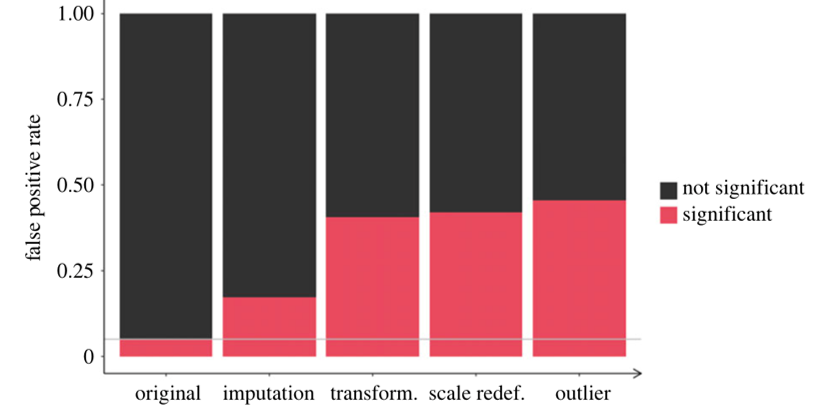
\includegraphics[width=1\linewidth,height=\textheight,keepaspectratio]{images/combining_hacks.png}
\end{center}

\begin{itemize}
\tightlist
\item
  Combining some of these hacks (\emph{aka questionable research
  practices}) can \textbf{raise false positive rates} from 5\% to
  \textgreater{} 50\%!
\item
  The logic of the p-value is therefore \textbf{corrupted} and
  ``\emph{renders the reported p-values essentially uninterpretable.}''
\end{itemize}

Stefan, A. M., \& Schönbrodt, F. D. (2023). Big little lies: A
compendium and simulation of p -hacking strategies. \emph{Royal Society
Open Science, 10}(2), 220346. \url{https://doi.org/10.1098/rsos.220346}

\textbf{Presenter Notes}: Even seemingly minor practices, e.g.,
selectively reporting results, stopping data collection once a
significant result appears, or testing multiple hypotheses without
proper correction, can have a huge effect. When these practices are
combined, they can inflate false positive rates dramatically, taking
them from the expected 5\% under proper statistical testing to over
50\%. This means that more than half of the reported significant
findings could be false alarms.

As a result, the logic of the p-value itself becomes corrupted. P-values
are supposed to indicate the probability of observing the data if the
null hypothesis is true. When questionable practices are used, this
interpretation no longer holds. In other words, it renders reported
p-values essentially uninterpretable, because they no longer reflect the
true probability of the observed effect under rigorous, unbiased
conditions.

\textbf{Instructor Notes}: Add.

\subsection{A note to remember}\label{a-note-to-remember}

\begin{tcolorbox}[enhanced jigsaw, arc=.35mm, bottomrule=.15mm, bottomtitle=1mm, breakable, colback=white, colbacktitle=quarto-callout-warning-color!10!white, colframe=quarto-callout-warning-color-frame, coltitle=black, left=2mm, leftrule=.75mm, opacityback=0, opacitybacktitle=0.6, rightrule=.15mm, title=\textcolor{quarto-callout-warning-color}{\faExclamationTriangle}\hspace{0.5em}{Warning}, titlerule=0mm, toprule=.15mm, toptitle=1mm]

The so-called ``hacks'' on the past few slides represent
\textbf{questionable research practices}. Do \textbf{not} try at home.

\end{tcolorbox}

\textbf{Presenter Notes}: I want to be clear before we move on: the way
the past slides were slide is deliberately sarcastic. It is meant to
show what can happen if researchers engage in questionable research
practices, like p-hacking, but it's \textbf{not a recommendation}.

\textbf{Instructor Notes}: Stress this point again d to potential
cultural differences in terms of processing sarcasm.

\subsection{\texorpdfstring{Practice \emph{p}-hacking
yourself}{Practice p-hacking yourself}}\label{practice-p-hacking-yourself}

\subsubsection{with the P-Hacker App}\label{with-the-p-hacker-app}

\url{http://shinyapps.org/apps/p-hacker/}

\pandocbounded{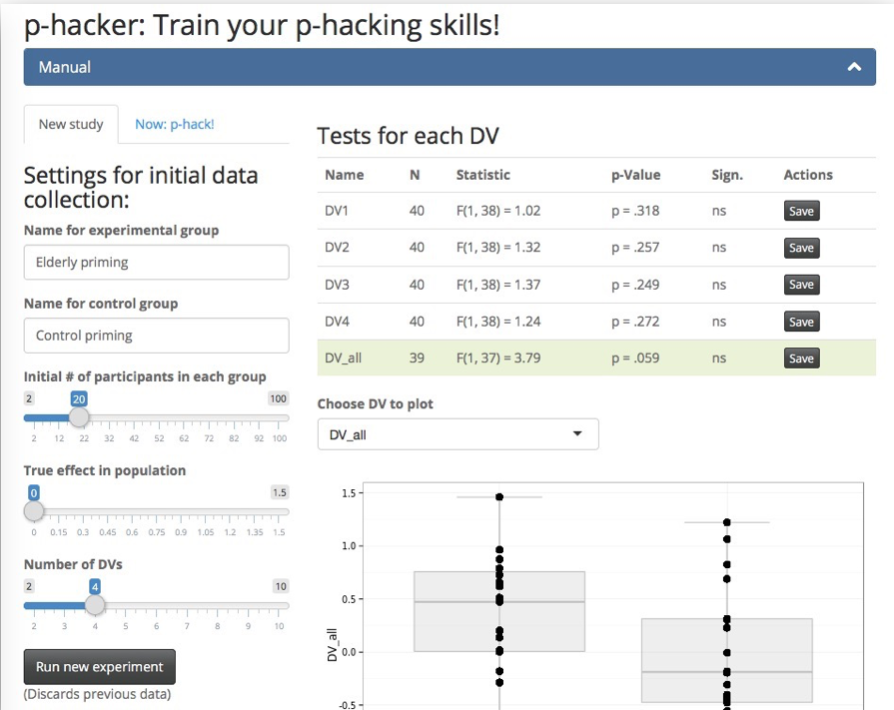
\includegraphics[keepaspectratio]{images/p-hacker-app.png}}

\subsection{Practical exercise 5}\label{practical-exercise-5}

\textbf{Scenario}: You are reviewing a study examining whether drinking
white tea improves short-term memory, where the researchers report:

\begin{itemize}
\item
  Hypothesis: \emph{White tea improves memory test scores.}
\item
  Sample size: 28 participants per group (tea-drinkers
  vs.~water-only-drinkers)
\item
  Results:

  \begin{itemize}
  \tightlist
  \item
    Effect was ``stronger in women'' (\emph{p} = 0.049)
  \item
    Effect ``even stronger when excluding two outliers'' (\emph{p} =
    0.044)
  \item
    No effect in men (\emph{p} = 0.31)
  \item
    Reaction time difference significant (\emph{p} = 0.046)
  \end{itemize}
\item
  Conclusion: \emph{The results show that white tea reliably improves
  cognitive performance.}
\end{itemize}

\textbf{Which potential p-hacking strategies are at play here?}

\textbf{Presenter Notes}: Let us get to work! I now have a task for you
to reflect on different biases and/ or questionable research practises.
Imagine that you are reviewing a study examining whether drinking white
tea improves short-term memory. In the report, you read the information
provided here. Which potential p-hacking strategies can you identify?

\textbf{Instructor Notes}: Possible answers can include:

\begin{itemize}
\item
  Large number of uncorrected comparisons with selective reporting
\item
  The conclusion variable does not match the original hypothesis
\item
  Research question too vague and non-directional given the analysis
\item
  Results report comparisons that are not specified in the research
  question
\item
  Many p values bunching just below 0.05
\item
  Lack of pre registration or analysis plan when claims are confirmatory
\item
  Outcome variables added that were not specified in the hypothesis:
  e.g., reaction time
\end{itemize}

\subsection{Practical exercise 5}\label{practical-exercise-5-1}

\textbf{Scenario}: You are reviewing a study examining whether drinking
white tea improves short-term memory, where the researchers report:

\begin{itemize}
\item
  Hypothesis: \emph{White tea improves memory test scores.}
\item
  Sample size: 28 participants per group (tea-drinkers
  vs.~water-only-drinkers)
\item
  Results:

  \begin{itemize}
  \tightlist
  \item
    Effect was ``stronger in \textbf{women}'' (\emph{p} =
    \textbf{0.049})
  \item
    Effect ``even stronger when excluding two outliers'' (\emph{p} =
    \textbf{0.044})
  \item
    No effect in \textbf{men} (\emph{p} = 0.31)
  \item
    \textbf{Reaction time} difference significant (\emph{p} =
    \textbf{0.046})
  \end{itemize}
\item
  Conclusion: The results show that white tea reliably improves
  \textbf{cognitive performance}.
\end{itemize}

\subsection{\texorpdfstring{Does this \emph{actually} happen in real
life?}{Does this actually happen in real life?}}\label{does-this-actually-happen-in-real-life}

Come on now. Surely not..? 😳

\begin{center}
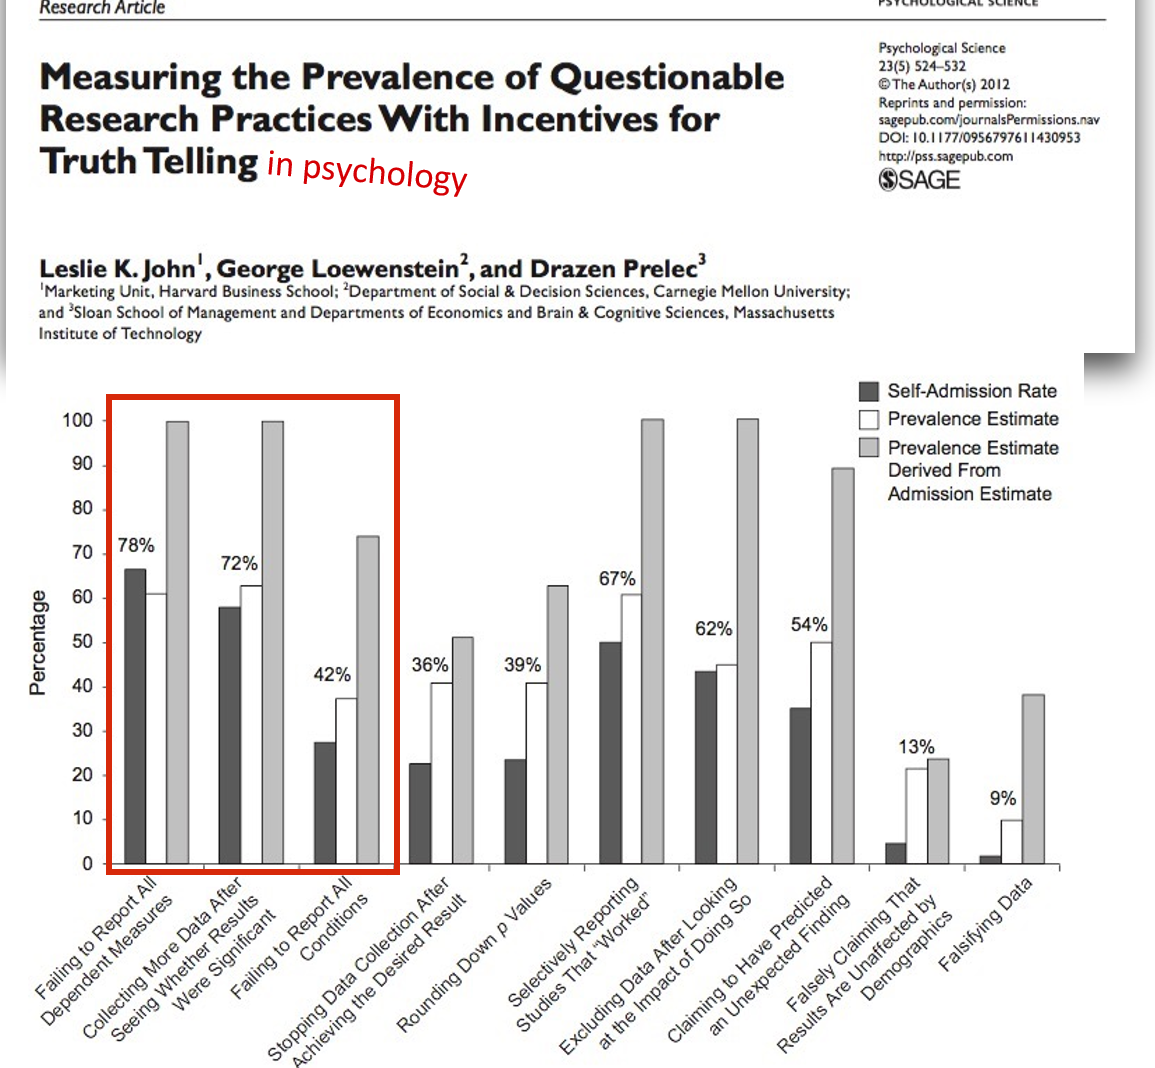
\includegraphics[width=1\linewidth,height=\textheight,keepaspectratio]{images/09_QRPs_Psychology.png}
\end{center}

John, L. K., Loewenstein, G., \& Prelec, D. (2012). Measuring the
prevalence of questionable research practices with incentives for truth
telling. \emph{Psychological science, 23}(5), 524-532.

\textbf{Presenter Notes}: At this point you might be thinking well ok,
we heard that p-hacking can be accidental. Surely then that means it
does not happen that often? Surely you can count the cases of this
happening on one hand. John and colleagues surveyed over 2,000
psychologists about their involvement in questionable research
practices.

In this survey, they asked respondents if they had ever failed to report
all outcome variables or they had ever collected more data after seeing
that the collected data did not result in the significant results they
wanted. The dark bar you see here are self-admissions rates, which for
these two practices in particular are above 70\%, which is extremely
high.

In their paper, they also used some estimation methods I won't go into
detail but just see that, well, over 70\% are \textbf{telling} us that
they engage in these practices, what would this percentage be in real
life? This is what is shown in the light grey bar, which for these two
practices specifically estimates the true percentage of engaging in
these two practices at almost 100\%, meaning that everyone has done this
at some point in their research career.

\textbf{Instructor Notes}: Quoting the relevant part of the paper: ``The
impact of truth-telling incentives on self-admissions of questionable
research practices was positive, and this impact was greater for
practices that respondents judged to be less defensible. Combining three
different estimation methods, we found that the percentage of
respondents who have engaged in questionable practices was surprisingly
high. This finding suggests that some questionable practices may
constitute the prevailing research norm.''

\subsection{.. and across fields?}\label{and-across-fields}

\begin{itemize}
\tightlist
\item
  Survey among 6,813 academic researchers in The Netherlands:
  \textbf{Self-reported prevalence of fabrication and falsification in
  the last 3 years}
\end{itemize}

\begin{center}
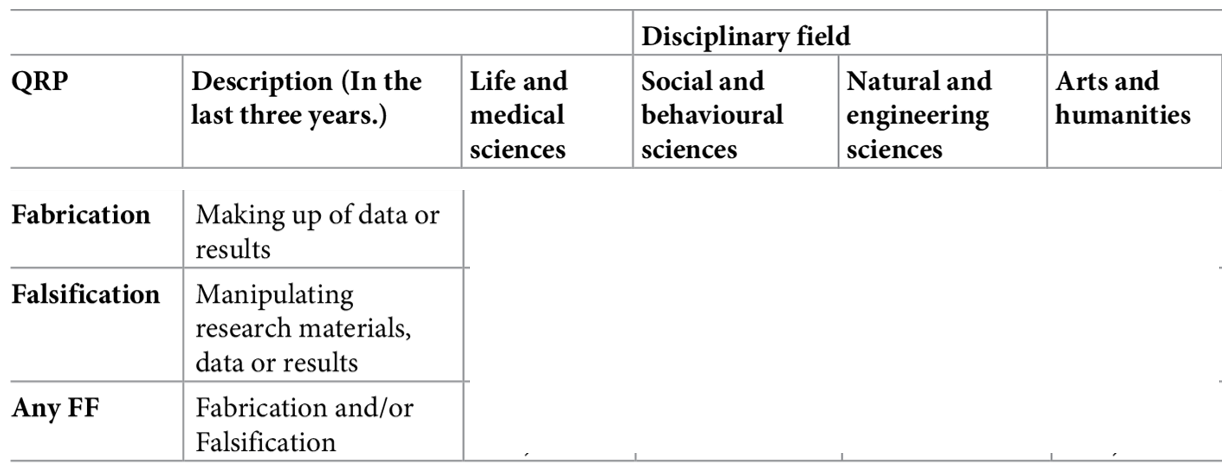
\includegraphics[width=0.5\linewidth,height=\textheight,keepaspectratio]{images/10_Self_Reported_blank.png}
\end{center}

Gopalakrishna, G., ter Riet, G., Vink, G., Stoop, I., Wicherts, J. M.,
\& Bouter, L. M. (2022). Prevalence of questionable research practices,
research misconduct and their potential explanatory factors: A survey
among academic researchers in The Netherlands. \emph{PLOS ONE, 17}(2),
e0263023. \url{https://doi.org/10.1371/journal.pone.0263023}

\textbf{Presenter Notes}: So far, we focused on questionable research
practices. Of course, there is also the next level, namely fabrication
and falsification, which both constitute outright scientific misconduct.
The authors conducted a large‑scale cross‑sectional survey (the National
Survey on Research Integrity) targeting academic researchers across all
disciplines and ranks in the Netherlands. Its aim was to estimate the
prevalence of fabrication and falsification and a range of questionable
research practices (QRPs) over the preceding three‑year period, and to
examine factors potentially associated with higher or lower engagement
in these behaviors. Over 6,800 researchers completed the survey. What
are your guesses here on the percentages they found?

\textbf{Instructor Notes}: Collect some guesses before moving on to
showing the solution.

\subsection{.. and across fields?}\label{and-across-fields-1}

\begin{itemize}
\tightlist
\item
  Survey among 6,813 academic researchers in The Netherlands:
  \textbf{Self-reported prevalence of fabrication and falsification in
  the last 3 years}
\end{itemize}

\begin{center}
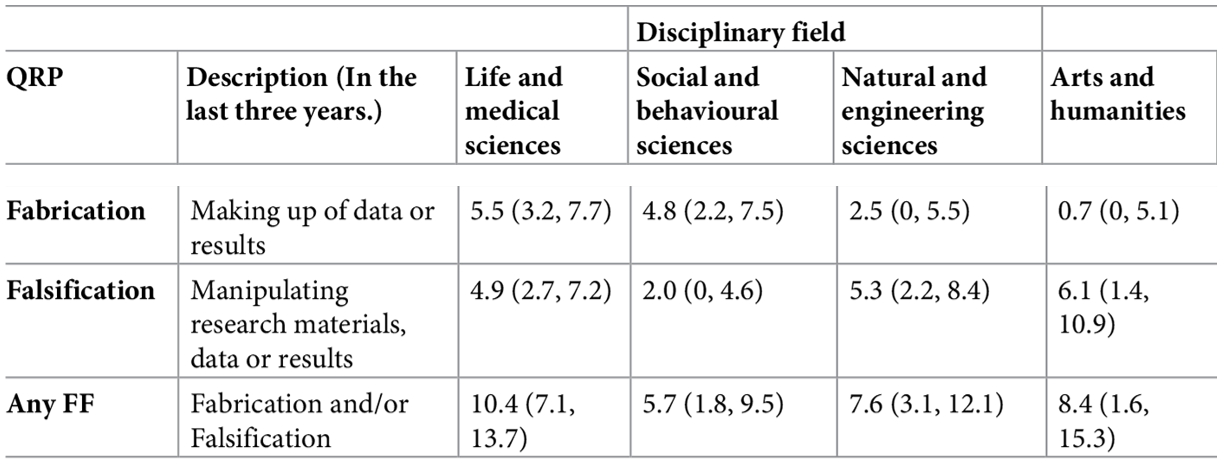
\includegraphics[width=0.5\linewidth,height=\textheight,keepaspectratio]{images/11_Self_Reported_QRP.png}
\end{center}

Gopalakrishna, G., ter Riet, G., Vink, G., Stoop, I., Wicherts, J. M.,
\& Bouter, L. M. (2022). Prevalence of questionable research practices,
research misconduct and their potential explanatory factors: A survey
among academic researchers in The Netherlands. \emph{PLOS ONE, 17}(2),
e0263023. \url{https://doi.org/10.1371/journal.pone.0263023}

\textbf{Presenter Notes}: The key findings from their study were quite
shocking. The prevalence of \textbf{fabrication}, aka making up data,
stands at about 4.3\% (with a 95\% confidence interval of 2.9 to 5.7\%),
while \textbf{falsification}, aka outright manipulating data, occurs at
roughly 4.2\% (95\% CI 2.8 to 5.6\%). These rates vary across
disciplines: for example, medical fields tend to report higher rates,
whereas arts and humanities report lower. Psychology shows a
self-reported fabrication rate of nearly 5\% and falsification around
2\%, indicating it is somewhat in the middle range.

When it comes to questionable research practices, which include 11 types
of behaviors assessed, the prevalence ranges widely. The least frequent
QRPs occur in about 0.6\% of respondents, while the most common QRP is
reported by as many as 17.5\% (95\% CI 16.4 to 18.7\%). Notably, over
half of the respondents (51.3\%) admitted to frequently engaging in at
least one QRP in the past three years.

Further analysis reveals that junior researchers, such as PhD
candidates, and male researchers have higher odds of frequently
reporting at least one QRP. On the other hand, individuals who strongly
subscribe to scientific norms, aka those that value honest research, and
those who believe that peer reviewers are likely to detect misconduct
show lower odds of engaging in misconduct or QRPs. Conversely,
researchers who experience higher publication pressure are more likely
to frequently engage in QRPs, with a 22\% increase in odds (OR
\textasciitilde1.22, 95\% CI 1.14 to 1.30).

\subsection{(Un)Intentional?}\label{unintentional}

\begin{itemize}
\tightlist
\item
  Intentional?

  \begin{itemize}
  \tightlist
  \item
    ``Evil researcher'' who only cares about his/her career and not at
    all about truth-seeking?
  \item
    „\emph{We urge the social science community to redefine p-hacking as
    a series of deceptive research practices rather than ones that are
    merely questionable.}`` (Craig et al., 2020)
  \end{itemize}
\item
  Unintentional?

  \begin{itemize}
  \tightlist
  \item
    Lack of education/knowledge?
  \item
    Wrong/uncritical standards of the field?
  \item
    Pushed by supervisors, reviewers, or editors? ➙
    \url{http://bulliedintobadscience.org/}
  \item
    \textbf{Simply being human?}
  \end{itemize}
\item
  Distorting effects on the published record are probably comparable,
  but the ethical evaluations differs strongly.
\end{itemize}

\textbf{Presenter Notes}: Summarising from the previous slides I showed,
we now know that questionable research practices and scientific
misconduct are extremely prevalent and frequent. The question here is:
why? Are we doing this \textbf{intentionally}, for example to publish
more papers and to advance our careers? Because we don't care about the
truth and about producing good quality, reliable research?

Or maybe this is all \textbf{unintentional}? Perhaps we did not fully
know that some of things we learnt from our PIs or supervisors are
considered bad practice? Maybe we are being convinced by supervisors?
Maybe there are just unclear standards of what is considered ``good
quality research'' in the field? Or maybe we are also just humans? We
already talked about inherent biases, but perhaps we also just make
mistakes or are unaware of our own weaknesses?

\section{Honest Errors}\label{honest-errors}

\subsection{Human errors and honest
mistakes}\label{human-errors-and-honest-mistakes}

\subsubsection{``90\% Excel-Gate''}\label{excel-gate}

\textbf{Presenter Notes}: In their 2010 paper Growth in a Time of Debt,
economists Carmen Reinhart and Kenneth Rogoff claimed that when
government debt exceeds 90\% of GDP, economic growth falls sharply.
Their findings strongly influenced debates about austerity policies.
However, in 2013, Thomas Herndon, Michael Ash, and Robert Pollin from
the University of Massachusetts--Amherst re-examined the data and found
serious flaws: an Excel coding error that excluded several countries. In
essence, what had happened was that when using a formula, the authors
had made a mistake when selecting the range of cells where to apply the
formula too. In this, they accidentally omitted some countries from the
calculations. The conclusion was that for advanced economies, when the
government gross debt exceeds about 90\% of GDP, annual real GDP growth
falls sharply. This conclusion informed policies in the respective
countries.

\textbf{Instructor Notes}: Details about the error: The omitted rows
related to countries with high debt and growth (for example Belgium)
that should have been part of the calculation. Because of this omission,
the reported average for the \textgreater90\% debt category was around
--0.1\% growth. Once corrected, the average growth rate for high-debt
countries rose from --0.1\% to about +2.2\%, showing no clear ``90\%
tipping point.'' The original authors later acknowledged the spreadsheet
error and issued a correction.

\subsection{Human errors and honest
mistakes}\label{human-errors-and-honest-mistakes-1}

\subsubsection{``90\% Excel-Gate'' - Lessons
learned}\label{excel-gate---lessons-learned}

\begin{tcolorbox}[enhanced jigsaw, arc=.35mm, bottomrule=.15mm, bottomtitle=1mm, breakable, colback=white, colbacktitle=quarto-callout-important-color!10!white, colframe=quarto-callout-important-color-frame, coltitle=black, left=2mm, leftrule=.75mm, opacityback=0, opacitybacktitle=0.6, rightrule=.15mm, title=\textcolor{quarto-callout-important-color}{\faExclamation}\hspace{0.5em}{Important}, titlerule=0mm, toprule=.15mm, toptitle=1mm]

The most important point of the story: The original authors
\textbf{shared their raw data}, which made it possible to
\textbf{correct} the honest mistake!

\end{tcolorbox}

\textbf{Presenter Notes}: The case became a landmark example of how data
errors, selective reporting, and methodological choices can mislead
economic policy, and of why transparency and replication are essential
in research. Only because the data were available, the mistake could be
found and corrected!

\subsection{Statistical errors}\label{statistical-errors}

\begin{center}
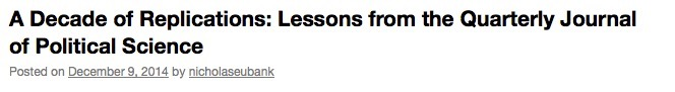
\includegraphics[width=1\linewidth,height=\textheight,keepaspectratio]{images/QuartelJournal_stat_analysis.png}
\end{center}

\begin{itemize}
\item
  Reproducible analysis \textbf{code and open data required} at
  submission - ``in-house checking'' in review process
\item
  54\% of all submissions had results in the paper that \textbf{did not
  match} the computed results from the code

  \begin{itemize}
  \tightlist
  \item
    Wrong signs, wrong labeling of regression coefficients, errors in
    sample sizes, wrong descriptive stats
  \end{itemize}
\end{itemize}

Eubank, N. (2016). Lessons from a decade of replications at the
quarterly journal of political science. \emph{PS: Political Science \&
Politics, 49}(2), 273-276
\url{https://doi.org/10.1017/S1049096516000196}

\textbf{Presenter Notes}: This is an interesting paper which looked at
code and data packages that were required at submission to the Quarterly
Journal of Political Science. They took the analysis code that and the
data that were submitted, reran the analysis and checked whether the
results matched what was described in the paper.

It finds that of the 24 empirical papers subjected to in-house
replication review since September 2012, only four packages did not
require any modifications. Most troubling, 14 packages (58\%) had
results in the paper that differed from those generated by the author's
own code. The authors identified a number of mistakes in the analysis
scripts that were submitted and in the results that were published, for
example that the wrong signs used for reporting, coefficients were
labelled the wrong way, descriptive statistics were imprecise or
incorrect.

Based on these experiences, this article presents a set of guidelines
for authors and journals for improving the reliability and usability of
replication packages.

\subsection{Statistical
inconsistencies}\label{statistical-inconsistencies}

\pandocbounded{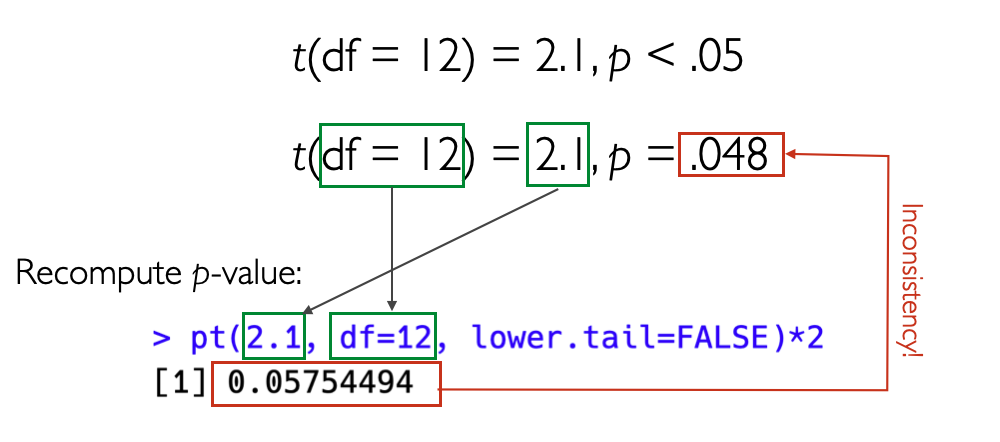
\includegraphics[keepaspectratio]{images/Statistical_inconsistency.png}}

\subsection{Statistical
inconsistencies}\label{statistical-inconsistencies-1}

\begin{center}

\includegraphics[width=0.1\linewidth,height=\textheight,keepaspectratio]{images/statcheck.png}
\end{center}

\begin{itemize}
\tightlist
\item
  Does the statistical conclusion change? ➙ „strong/gross
  inconsistency``
\item
  Psychology:

  \begin{itemize}
  \tightlist
  \item
    16,695 scanned papers with \textbf{statcheck tool} (Nuijten et al.,
    2015)
  \item
    50\% of papers contain statistical inconsistencies
  \item
    13\% contained \textbf{strong errors} (i.e., where the statistical
    conclusion changes).
  \end{itemize}
\item
  Economics

  \begin{itemize}
  \tightlist
  \item
    3,677 scanned papers with DORIS tool (Bruns et al., 2023)
  \item
    36\% of papers contain statistical inconsistencies
  \item
    15\% contained strong errors (i.e., where the statistical conclusion
    changes).
  \end{itemize}
\item
  Other fields (e.g.~Sociology):

  \begin{itemize}
  \tightlist
  \item
    Not even (automatically) checkable, due to unstandardized reporting
    practices.
  \end{itemize}
\item
  \ldots{} and these are only the {detected} errors of {one} type (stat.
  inconsistency)!
\end{itemize}

Nuijten et al.~(2016). The prevalence of statistical reporting errors in
psychology (1985--2013). \emph{Behavior research methods, 48}(4),
1205-1226. \url{https://doi.org/10.3758/s13428-015-0664-2}. Bruns et
al.(2023). Statistical reporting errors in economics {[}Preprint{]}.
MetaArXiv. \url{https://doi.org/10.31222/osf.io/mbx62}

\textbf{Presenter Notes}: Researchers have also examined how often
published psychology papers contain statistical errors. Using the
\emph{Statcheck} tool (Nuijten et al., 2015), over 16,000 papers were
automatically scanned to compare reported test statistics with their
p-values. The results were worrying: about 50\% of papers contained at
least one statistical inconsistency, and around 13\% had serious errors,
meaning the reported statistical conclusion (for example, whether a
result was ``significant'') would actually change if calculated
correctly.

More recent work by Crüwell et al.~(2022) found that the numerical
results in fewer than 30\% of papers can be fully reproduced, even when
all the information needed is available.

I want to point out here that these are only errors of the statistical
type, other types of errors were not examined here. I think you see the
picture that I am painting here and I am hoping to get across that these
are some serious challenges to research.

\subsection{Reproducibility Success}\label{reproducibility-success}

\begin{itemize}
\tightlist
\item
  Numerical results of less than 30\% of papers can be
  \textbf{reproduced} (Crüwell et al., 2022)
\item
  TODO: Add the current meta-studies by Kraehmer et al
\end{itemize}

\subsection{What does this all mean?}\label{what-does-this-all-mean}

\textbf{Bias + (may unintentional) \emph{p}-hacking + human (honest)
mistakes = untrustworthy research findings?}

\begin{tcolorbox}[enhanced jigsaw, arc=.35mm, bottomrule=.15mm, bottomtitle=1mm, breakable, colback=white, colbacktitle=quarto-callout-note-color!10!white, colframe=quarto-callout-note-color-frame, coltitle=black, left=2mm, leftrule=.75mm, opacityback=0, opacitybacktitle=0.6, rightrule=.15mm, title=\textcolor{quarto-callout-note-color}{\faInfo}\hspace{0.5em}{Note}, titlerule=0mm, toprule=.15mm, toptitle=1mm]

\begin{itemize}
\tightlist
\item
  Published findings across fields to be viewed with \textbf{caution}?
\item
  ``We know'' --\textgreater{} \textbf{``We \emph{think} we know''}?
\item
  More research to \textbf{verify} existing ``truths''?
\end{itemize}

\end{tcolorbox}

\textbf{Presenter Notes}: Taking all of this together, where does this
leave us? We have several elements which, as we have explored in the
last few slides, contribute to non-robust research. We have different
types of biases, accidential or not so accidental p-hacking, and we have
the human component of just making mistakes from time to time in the
process. What conclusions can we draw about research, then?

Perhaps there should be more caution around published papers across
fields and we should not view findings as the ultimate truth, just
because they were published? Perhaps we should also shift from ``we
know'' to ``we think we know'' pending further investigations and
perhaps pending replication? And finally, perhaps our efforts should
also go into checking these so-called truths we think exist in the
academic world and perform more replication studies?

\textbf{Instructor Notes}: This is a critical reflection moment, give
enough time between this slide and the next slide for learners to digest
and integrate what they learned.

\subsection{A romanticized idea of
research?}\label{a-romanticized-idea-of-research}

\textbf{Presenter Notes}: In other words, perhaps we have a romanticized
view of research? Typically we think of research as something along the
following lines: The smartest heads in the world immerse themselves into
a research topic for years. In that process, they become the experts,
nobody knows more about that topic.The boundaries of knowledge have been
pushed forward. When the researchers are confident in their findings,
they publish them in the best scientific journals, with the highest
standards of quality, rigor, and integrity.

\textbf{Instructor Notes}: Encourage a mental shift by contrasting how
we used to think about research and the current status quo discussed
over the past slides. Prepare the ``stage'' for a new approach to
research and guide your learners towards the question of ``but then how
can we do research differently''?

\subsection{Going even further: The perpetuating role of
AI}\label{going-even-further-the-perpetuating-role-of-ai}

Emsley, R. (2023). ChatGPT: These are not hallucinations - they're
fabrications and falsifications. \emph{Schizophrenia, 9}(1), 52.
Lautrup, A. D., Hyrup, T., Schneider-Kamp, A., Dahl, M., Lindholt, J.
S., \& Schneider-Kamp, P. (2023). Heart-to-heart with ChatGPT: the
impact of patients consulting AI for cardiovascular health advice.
\emph{Open Heart, 10}(2). Shekar, S., Pataranutaporn, P., Sarabu, C.,
Cecchi, G. A., \& Maes, P. (2025). People Overtrust AI-Generated Medical
Advice despite Low Accuracy. \emph{NEJM AI, 2}(6), AIoa2300015.

\textbf{Presenter Notes}: Thinking about how mistakes happen, how
accidental p-hacking happens, how there is pressure to publish positive
results, how we are, to some extent, victims of our own biases without
noticing, I think you get an image of the low credibility of research
that is currently out there. Now we are also facing a new challenge in
the wake of artificial intelligence. We know that ChatGPT and other
large language models are routinely used by people to, for example,
obtain medical advice. Given what we heard before, how accurate do you
believe this information provided by the chatbots is? Papers demonstrate
by now that the accuracy is low, yet people turn to ChatGPT for medical
advice. We also know about so-called hallucinations of ChatGPT. Some
researchers view this as the ``modern'' form of falsification and
fabrication, just like we discussed in the context of scientific
misconduct. But what if the research feeding into this advice that
chatbots provide and the ``papers'' they are suggesting to you for your
essay are already of low quality? Is AI then not simply distributing
non-credible and flawed research, without the warning message that this
might be the case?

\textbf{Instructor Notes}: Bonus slide depending on the interest of your
learners.

\subsection{}\label{section}

Thesis:

Our current incentives foster questionable research practices, which
decrease the truth value of our shared knowledge.

What is good for the individual careers of researchers leads to a
collective fiasko.

Researchers who do it right (i.e., high power, no QRPs, transparency)
have a clear competitive disadvantage.

Anti-Thesis:

Society pays for us that we generate valid and robust knowledge.

Our incentives should be chosen in a way that they foster good science.

Researchers who do it right should be supported and promoted.

\subsection{Now what?}\label{now-what}

\begin{center}
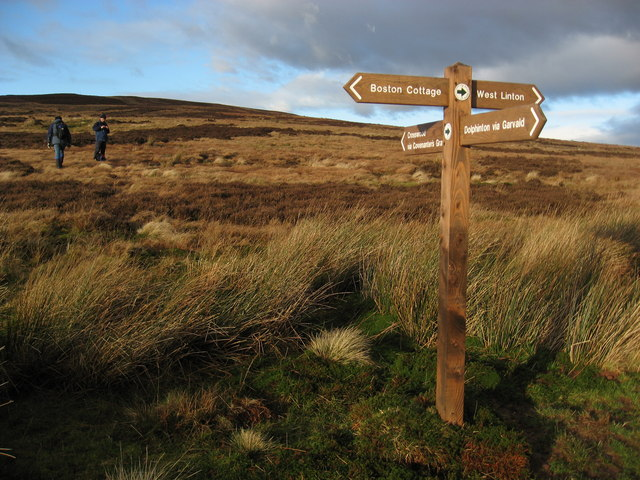
\includegraphics[width=1\linewidth,height=\textheight,keepaspectratio]{images/crossroads.png}
\end{center}

This image was taken from the
\href{https://www.geograph.org.uk/}{Geograph project collection}. The
copyright on this image is owned by Chris Martin and is licensed for
reuse under the Creative Commons Attribution-ShareAlike 2.0 license.

\textbf{Presenter Notes}: At this point, you might think that research
is doomed. That perhaps humanity is doomed along with it. Despite
everything we talked about today, this could not be further from the
truth. There are different approaches to research, which mitigate many
of these challenges we discussed today. These approaches have the aim to
raise scientific standards and the quality of research, so that society
and researchers can trust the published work.

\subsection{A new way of doing
research}\label{a-new-way-of-doing-research}

\textbf{Open Research} \emph{aka} \textbf{A scientific framework for the
21. century}

\textbf{Presenter Notes}: What I mean with this alternative approach is
Open Research, which is a framework for how to do research in the 21st
century. We will have the entire following session to dive deeper into
what Open Research even means or how it can possibly make research more
credible. The focus of the next session will all be about how Open
Research can change the game.

\textbf{Instructor Notes}: Make the shift from describing the problem,
threats and challenges of research to a more solution-focused framework
of reference.

\section{To be continued \ldots{}}\label{to-be-continued}

\textbf{Presenter Notes}: What exactly Open Research entails will be the
focus of the following session. \textbf{Instructor Notes}: Emphasize
that Open Research will be discussed in great detail in the upcoming
session and that today's focus were on understanding the current
problems in research.

\subsection{Reflection activity}\label{reflection-activity}

\textbf{One-minute paper}: Imagine you would have to explain the current
challenges in research you heard about today to a friend. Write down
what you would say to them.

\textbf{Presenter Notes}: Wrapping things up: Imagine you would have to
explain the current challenges in research you heard about today to a
friend. Write down what you would say to them.

\textbf{Instructor Notes}: Ask for 2-3 volunteers willing to share their
papers in class. Alternatively, have your learners either hand you in
the pieces of paper they wrote this on, or ask your learners to send you
their one-minute-papers by email.

\subsection{Take-home message}\label{take-home-message}

\textbf{What are you taking away from today?}

\subsection{Take-home message}\label{take-home-message-1}

\textbf{What are you taking away from today?}

\begin{tcolorbox}[enhanced jigsaw, arc=.35mm, bottomrule=.15mm, bottomtitle=1mm, breakable, colback=white, colbacktitle=quarto-callout-tip-color!10!white, colframe=quarto-callout-tip-color-frame, coltitle=black, left=2mm, leftrule=.75mm, opacityback=0, opacitybacktitle=0.6, rightrule=.15mm, title=\textcolor{quarto-callout-tip-color}{\faLightbulb}\hspace{0.5em}{Remember: There are solutions!}, titlerule=0mm, toprule=.15mm, toptitle=1mm]

Research is \textbf{not ``doomed'' - on the contrary}. More on this in
the \emph{next} session!

\end{tcolorbox}

\section{\texorpdfstring{Thanks! }{Thanks!  }}\label{thanks}

See you next class :)

\subsection{Additional exercises: Replicability and
reproducibility}\label{additional-exercises-replicability-and-reproducibility}

Decide whether each scenario in the following slides is an example of
\textbf{reproducibility} or \textbf{replicability}.

\textbf{Presenter Notes}: Add script for slide here. \textbf{Instructor
Notes}: Think pair share.

\subsection{Scenario 1}\label{scenario-1}

\textbf{A computational neuroscientist reruns a published fMRI analysis
using the original dataset and Python scripts to verify the reported
brain activation patterns.}

\textbf{Presenter Notes}: Add script for slide here. \textbf{Instructor
Notes}: Correct answer: Reproducibility

\subsection{Scenario 2}\label{scenario-2}

\textbf{An environmental scientist repeats a field experiment on soil
nutrient levels using the same sampling protocol at a different site.}

\textbf{Presenter Notes}: Add script for slide here. \textbf{Instructor
Notes}: Correct answer: Replicability

\subsection{Scenario 3}\label{scenario-3}

\textbf{A linguist reanalyzes a corpus of historical texts using the
same annotation guidelines and code to verify reported patterns of
syntactic structures.}

\textbf{Presenter Notes}: Add script for slide here. \textbf{Instructor
Notes}: Correct answer: Reproducibility

\subsection{Scenario 4}\label{scenario-4}

\textbf{A psychology lab replicates a social behavior experiment using
new participants from a different cultural background.}

\textbf{Presenter Notes}: Add script for slide here. \textbf{Instructor
Notes}: Correct answer: Replicability

\subsection{Psychology: The Replication Database by
FORRT}\label{psychology-the-replication-database-by-forrt}

\begin{itemize}
\tightlist
\item
  Collects replication results across different psychological fields
\item
  Provide detailed overview of the original findings and the replication
  outcomes
\end{itemize}

\begin{center}
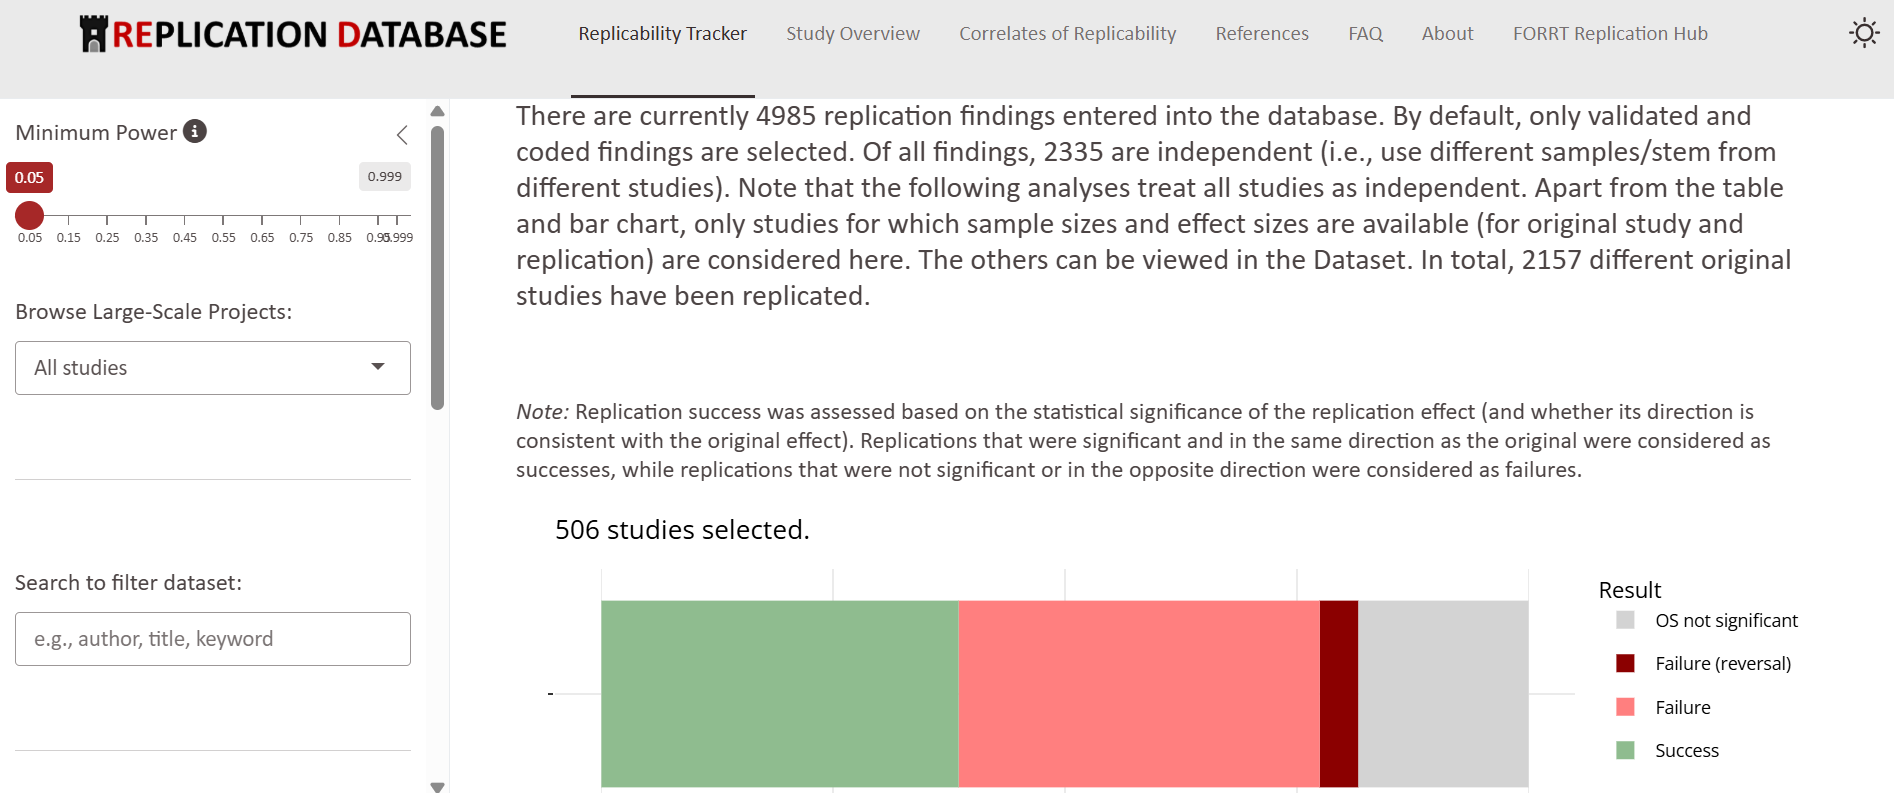
\includegraphics[width=1\linewidth,height=\textheight,keepaspectratio]{images/FORRT_Replication_Database.png}
\end{center}

\textbf{FORRT Replication Database}
(\url{https://forrt-replications.shinyapps.io/fred_explorer/})

\subsection{References}\label{references}

\protect\phantomsection\label{refs}
\begin{CSLReferences}{1}{0}
\bibitem[\citeproctext]{ref-andersonTaxonomyLearningTeaching2001}
Anderson, L. W., \& Krathwohl, D. R. (2001). \emph{A taxonomy for
learning, teaching, and assessing : A revision of {Bloom}'s taxonomy of
educational objectives : Complete edition}. Addison Wesley Longman, Inc.

\bibitem[\citeproctext]{ref-bloom1955NormativeStudy1956}
Bloom, B. S. (1956). The 1955 {Normative Study} of the {Tests} of
{General Educational Development}. \emph{The School Review},
\emph{64}(3), 110--124. \url{https://doi.org/10.1086/442296}

\bibitem[\citeproctext]{ref-craigUsingRetractedJournal2020}
Craig, R., Cox, A., Tourish, D., \& Thorpe, A. (2020). Using retracted
journal articles in psychology to understand research misconduct in the
social sciences: {What} is to be done? \emph{Research Policy},
\emph{49}(4), 103930. \url{https://doi.org/10.1016/j.respol.2020.103930}

\bibitem[\citeproctext]{ref-cruwellWhatsBadgeComputational2022}
Crüwell, S., Apthorp, D., Baker, B. J., Colling, L. J., Elson, M.,
Geiger, S. J., Lobentanzer, S., Monéger, J., Patterson, A., Schwarzkopf,
D. S., Zaneva, M., \& Brown, N. J. L. (2022). \emph{What's in a badge?
{A} computational reproducibility investigation of the {Open Data} badge
policy in one {Issue} of {Psychological Science}}. PsyArXiv.
\url{https://doi.org/10.31234/osf.io/729qt}

\bibitem[\citeproctext]{ref-schmidtCreatingSPACEEvolve2021}
Schmidt, R., Curry, S., \& Hatch, A. (2021). Creating {SPACE} to evolve
academic assessment. \emph{eLife}, \emph{10}, e70929.
\url{https://doi.org/10.7554/eLife.70929}

\end{CSLReferences}

\section{Additional slides TO
REMOVE?}\label{additional-slides-to-remove}

\subsection{What published research can be replicated/reproduced?
REMOVE}\label{what-published-research-can-be-replicatedreproduced-remove}

{\def\LTcaptype{none} % do not increment counter
\begin{longtable}[]{@{}
  >{\raggedright\arraybackslash}p{(\linewidth - 4\tabcolsep) * \real{0.6400}}
  >{\raggedright\arraybackslash}p{(\linewidth - 4\tabcolsep) * \real{0.1800}}
  >{\raggedright\arraybackslash}p{(\linewidth - 4\tabcolsep) * \real{0.1800}}@{}}
\toprule\noalign{}
\begin{minipage}[b]{\linewidth}\raggedright
Field
\end{minipage} & \begin{minipage}[b]{\linewidth}\raggedright
Success
\end{minipage} & \begin{minipage}[b]{\linewidth}\raggedright
Failure
\end{minipage} \\
\midrule\noalign{}
\endhead
\bottomrule\noalign{}
\endlastfoot
OSC (2015) -- Psychology & 36\% & 64\% \\
Chang \& Li (2015) -- Economics (67 papers, 29 papers replicated) & 43\%
& 57\% \\
Camerer 2016 -- Econ laboratory & 61\% & 39\% \\
Camerer combined Social Sci & 62\% & 38\% \\
Begley \& Ellis (2012) -- Cancer Research & 11\% & 89\% \\
Prinz et al.~(2011) -- Pharmaceutical research & 35\% & 65\% \\
Cova et al.~(2018) -- x-philosophy & 70\% & 30\% \\
Protzko et al.~(2023) -- Social & 86\% & 14\% \\
\end{longtable}
}

\subsection{Why should we trust
researchers?}\label{why-should-we-trust-researchers}

\begin{center}
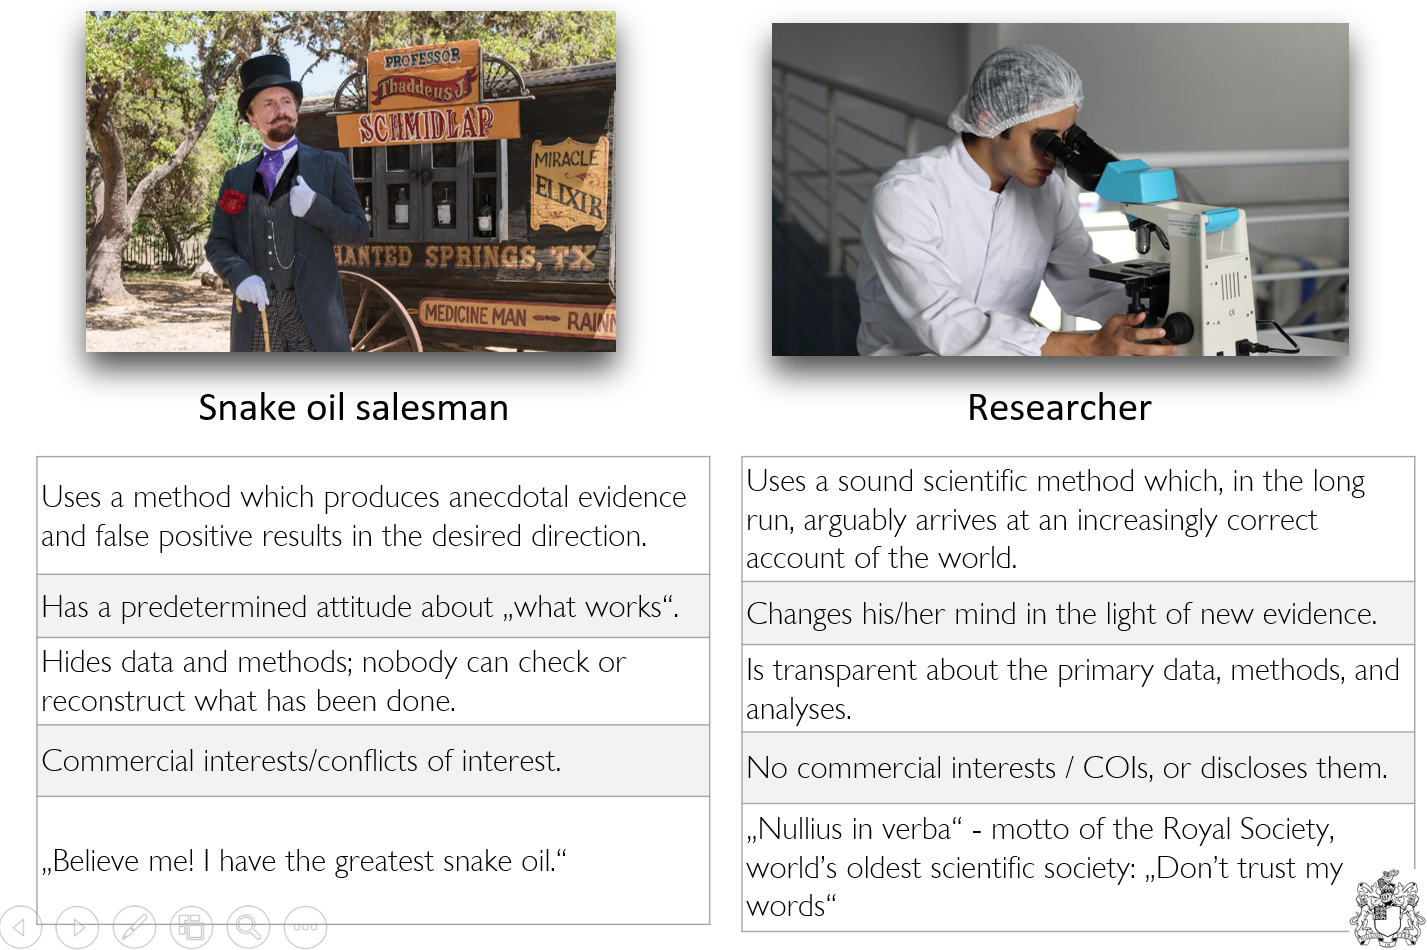
\includegraphics[width=1\linewidth,height=\textheight,keepaspectratio]{images/01_snakesman_researcher.png}
\end{center}

\subsection{\ldots right? MOVE}\label{right-move}

\begin{center}
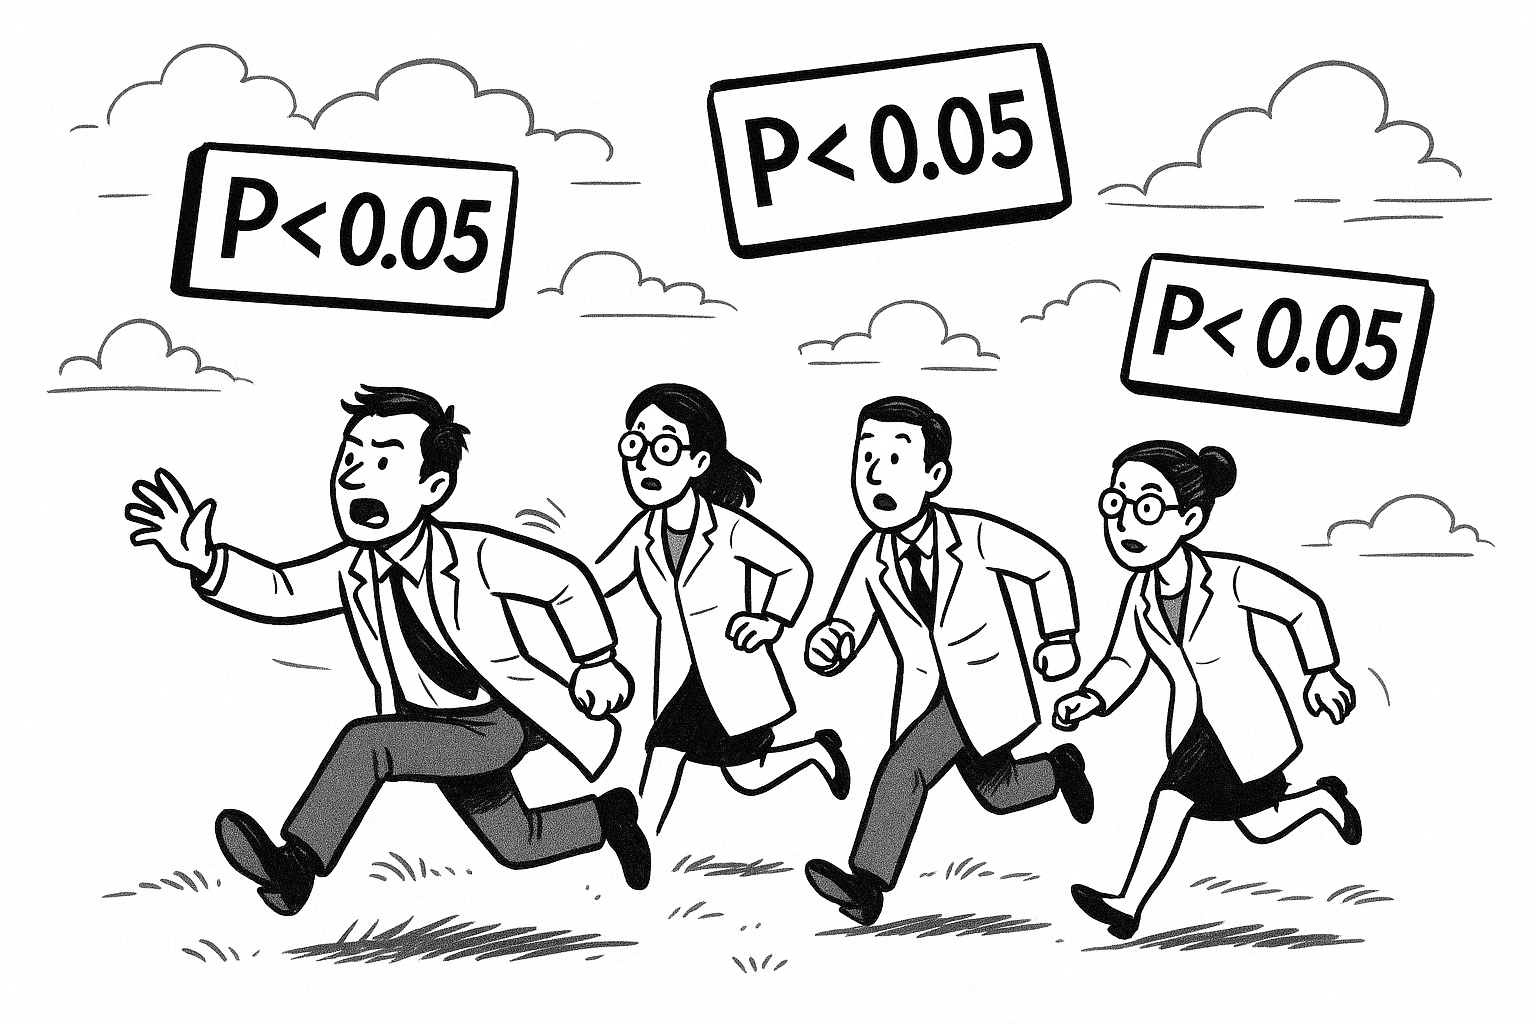
\includegraphics[width=0.5\linewidth,height=\textheight,keepaspectratio]{images/07_holy_grail.png}
\end{center}

\subsection{Decide where to add - maybe not
needed?}\label{decide-where-to-add---maybe-not-needed}

\textbf{Ideal scenario: Balancing the desire to stay truthful to
research with the necessity to publish?}




\end{document}
